% % % % % % % % % % % % % % % % % % % % % % % % % % % % % % % % % % % % % % % %
% LaTeX4EI Template for Cheat Sheets                                Version 1.0
%
% Authors: Emanuel Regnath, Martin Zellner
% Contact: info@latex4ei.de
% Encode: UTF-8, tabwidth = 4, newline = LF
% % % % % % % % % % % % % % % % % % % % % % % % % % % % % % % % % % % % % % % %


% ======================================================================
% Document Settings
% ======================================================================

% possible options: color/nocolor, english/german, threecolumn
% defaults: color, english
\documentclass[english]{latex4ei/latex4ei_sheet}

% set document information
\title{Technische Felder\\ und Wellen}
\author{Markus Kaschke, Johannes Kunz}					% optional, delete if unchanged
\myemail{info@latex4ei.de}			% optional, delete if unchanged
\mywebsite{www.latex4ei.de}			% optional, delete if unchanged


\let\T\relax
\DeclareMathOperator{\T}{\textsf{\textit{T}}}		% Zufallsvariable X
\DeclareMathOperator{\Bias}{Bias}		% Zufallsvariable X
\DeclareMathOperator{\argmax}{argmax}

\DeclareMathOperator{\rang}{rang}
\renewcommand{\vec}[1]{\underline{\boldsymbol{#1}}}
%\renewcommand{\vec}[1]{\boldsymbol{#1}}



\newcommand{\x}{\textit{x}}
\newcommand{\vx}{\underline{\textbf{\textit{x}}}}
\newcommand{\VX}{\underline{\textbf{\textit{X}}}}

\newcommand{\y}{\textit{y}}
\newcommand{\vy}{\underline{\textbf{\textit{y}}}}
\newcommand{\VY}{\underline{\textbf{\textit{Y}}}}


\newcommand{\VA}{\underline{\textit{A}}}
\newcommand{\A}{\textit{A}}
\newcommand{\va}{\underline{\textbf{\textit{a}}}}

\newcommand{\VB}{\underline{\textit{B}}}
\newcommand{\danger}[1]{\textcolor{red}{#1}}

\newcommand{\comment}[1]{\textcolor{red}{#1}}

\usepackage{multirow}


% ======================================================================
% Begin
% ======================================================================
\begin{document}

\IfFileExists{git.id}{\input{git.id}}{}
\ifdefined\GitRevision\mydate{\GitNiceDate\ (git \GitRevision)}\fi
% Title
% ----------------------------------------------------------------------
\maketitle   % requires ./img/Logo.pdf

% Section
% ----------------------------------------------------------------------
\section{Math}
% ======================================================================

\begin{sectionbox}
	\begin{tabular}{@{}llll}
		$\pi \approx \num{3,14159}$ & $e \approx \num{2,71828}$ & $\sqrt{2} \approx \num{1,414}$ & $\sqrt{3} \approx \num{1,732}$ \\
	\end{tabular}

	\textbf{Binome, Trinome}\\
	$(a\pm b)^2 = a^2 \pm 2ab + b^2$ \hfill $a^2 - b^2 = (a-b)(a+b)$\\
	$(a \pm b)^3 = a^3 \pm 3a^2b + 3ab^2 \pm b^3$\\
	$(a+b+c)^2 = a^2 + b^2 + c^2 + 2ab + 2ac + 2bc$
	\\[0.5em]
	\textbf{Folgen und Reihen}\\
	$\underset{\text{Aritmetrische Summenformel}}{\sum \limits_{k=1}^{n} k = \frac{n (n+1)}{2}}$ \quad $\underset{\text{Geometrische Summenformel}}{\sum \limits_{k=0}^{n} q^k = \frac{1 - q^{n+1}}{1-q}}$ \quad $\underset{\text{Exponentialreihe}}{\sum\limits_{n = 0}^{\infty} \frac{\cx z^n}{n!} = e^{\cx z}}$\\
	\\[0.5em]
	\textbf{Mittelwerte} \quad ($\sum$ von $i$ bis $N$) \hfill {\small (Median: Mitte einer geordneten Liste)}\\
	\begin{tabular*}{\columnwidth}{@{\extracolsep\fill}l@{\quad\ $\ge$}l@{\quad\ $\ge$}l}
	$\underset{\text{Arithmetisches}}{\ol x_{\ir{ar}} = \frac{1}{N} \sum x_i}$ & $\underset{\text{Geometrisches Mittel}}{\ol x_{\ir{geo}} = \sqrt[N]{ \prod x_i }}$ & $\underset{\text{Harmonisches}}{\ol x_{\ir hm} = }\frac{N}{\sum \frac{1}{x_i}}$\\
	\end{tabular*}
	\\[0.5em]
	\textbf{Ungleichungen:} \hfill Bernoulli-Ungleichung:  $(1+x)^n \ge 1+nx$\\
	$\underset{\text{Dreiecksungleichung}}{\big|\! \abs{x}- \abs{y}\!\big| \le \abs{x \pm y} \le \abs{x} + \abs{y}}$ \hfill
	$\underset{\text{Cauchy-Schwarz-Ungleichung}}{\left| \vec x^\top \bdot \vec y \right| \le \| \vec x\| \cdot \| \vec y\|}$
	\\[0.5em]
	\textbf{Mengen:} De Morgan: $\overline{A \capdot B} = \overline{A} \cupplus \overline{B}$ \hfill $\overline{A \cupplus B} = \overline{A} \capdot \overline{B}$
\end{sectionbox}

\begin{sectionbox}
	\subsection[Exp. und Log.]{Exp. und Log.\ \ $e^x := \lim\limits_{n \rightarrow \infty} \left( 1 + \frac{x}{n} \right)^n \hfill e \approx 2,71828$}
	\begin{tabular*}{\columnwidth}{@{\extracolsep\fill}lll@{}}
		$a^x = e^{x \ln a}$ & $\log_a x = \frac{\ln x}{\ln a}$ & $\ln x \le x -1$\\
		$\ln(x^{a}) = a \ln(x)$ & $\ln(\frac{x}{a}) = \ln x - \ln a$ & $\log(1) = 0$\\
	\end{tabular*}
\end{sectionbox}


\begin{sectionbox}
	\subsection[Matrizen]{Matrizen $\ma A \in\mathbb{K}^{m \times n}$}
	$\ma A=(a_{ij}) \in \mathbb K^{m\times n}$ hat $m$ Zeilen (Index $i$) und $n$ Spalten (Index $j$)
	\begin{tabular*}{\columnwidth}{ll}
	$(\ma A + \ma B)^\top = \ma A^\top + \ma B^\top$ & $(\ma A \cdot \ma B)^\top = \ma B^\top \cdot \ma A^\top$\\
	${(\ma A^\top)}^{-1} = {(\ma A^{-1})}^\top$ & $(\ma A \cdot \ma B)^{-1} = \ma B^{-1}\ma A^{-1}$
	\end{tabular*}
	$\dim \mathbb K = n = \rang\ma A + \dim\ker\ma A$ \qquad $\rang\ma A = \rang\ma A^\top$


	\subsubsection{Quadratische Matrizen $A \in \mathbb{K}^{n \times n}$}
	regulär/invertierbar/nicht-singulär $\Leftrightarrow \det (\ma A) \ne 0 \Leftrightarrow \rang\ma A = n$\\
	singulär/nicht-invertierbar $\Leftrightarrow \det (\ma A) = 0 \Leftrightarrow \rang\ma A \ne n$\\
	orthogonal $\Leftrightarrow \ma A^\top=\ma A^{-1} \Ra \det(\ma A) = \pm 1$\\
	symmetrisch: $\ma A=\ma A^\top$ \qquad schiefsymmetrisch: $\ma A=-\ma A^\top$
	%\item hermitsch: $\ma A=\overline{\ma A}^\top$, unitär:$\ma A^{-1} = \overline{\ma A}^\top$


	\subsubsection[Determinante]{Determinante von $\ma A\in \mathbb K^{n\times n}$: $\det(\ma A)=|\ma A|$}
	$\det\mat{ \ma A & \ma 0 \\ \ma C& \ma D }= \det\mat{ \ma A & \ma B \\ \ma 0 & \ma D } = \det(\ma A)\det(\ma D)$ \\
	\begin{tabular*}{\columnwidth}{@{\extracolsep\fill}ll}
	$\det(\ma A) = \det(\ma A^T)$ & $\det(\ma A^{-1}) = \det(\ma A)^{-1}$
	\end{tabular*}
	$\det(\ma A\ma B) = \det(\ma A)\det(\ma B) = \det(\ma B)\det(\ma A) = \det(\ma B\ma A)$\\
	Hat $\ma A$ 2 linear abhäng. Zeilen/Spalten $\Rightarrow |\ma A|=0$ \\

	\subsubsection{Eigenwerte (EW) $\lambda$ und Eigenvektoren (EV) $\underline v$}
	\begin{emphbox}
		\large $\ma A \vec v = \lambda \vec v$ \quad\ $\det \ma A = \prod \lambda_i$ \quad\ $\Sp \ma A = \sum a_{ii} = \sum \lambda_i$
	\end{emphbox}
	Eigenwerte: $\det(\ma A - \lambda \ma 1) = 0$ Eigenvektoren: $\ker(\ma A - \lambda_i \ma 1) = \vec v_i$\\
	EW von Dreieck/Diagonal Matrizen sind die Elem. der Hauptdiagonale.


	\subsubsection{Spezialfall $2 \times 2$ Matrix $A$}
	\parbox{3cm}{ $\det(\ma A) = ad-bc$ \\ $\Sp(\ma A) = a+d$ } $\mat{a & b\\ c & d}^{-1} = \frac{1}{\det \ma A} \mat{d & -b\\ -c& a}$\\
	$\lambda_{1/2} = \frac{\Sp \ma A}{2} \pm \sqrt{ \left( \frac{\mathrm{sp} \ma A}{2} \right)^2 - \det \ma A }$

	\subsubsection{Differentiation}
	$\frac{\partial \vec x^\top \vec y}{\partial \vec x} = \frac{\partial \vec y^\top \vec x}{\partial \vec x} = \vec y$\qquad
	$\frac{\partial \vec x^\top \ma A \vec x}{\partial \vec x} = (\ma A + \ma A^\top)\vec x$ \\
	$\frac{\partial \vec x^\top \ma A \vec y}{\partial \ma A} = \vec x \vec y^\top$ \qquad $\frac{\partial \det( \ma B \ma A \ma C )}{\partial \ma A} = \det(\ma B \ma A \ma C) \left( \ma A^{-1} \right)^\top$
\end{sectionbox}



%\begin{sectionbox}
%	\subsubsection{Ableitungsregeln ($\forall \lambda, \mu \in \mathbb R$)}
%	\begin{tabular}{@{}l@{\quad}ll@{}}
%		Linearität: & $(\lambda f + \mu g)' (x) = \lambda f'(x) + \mu g'(x_0)$  \\
%		Produkt: & $(f \cdot g)'(x) = f'(x) g(x) + f(x) g'(x)$\\
%		Quotient: & $\left(\frac{f}{g}\right)' (x) = \frac{g(x)f'(x) -f(x) g'(x)}{g(x)^2}$ \quad $\left(\frac{\text{NAZ}-\text{ZAN}}{\text{N}^2}\right)$\\
%		Kettenregel & $\left( f\bigl(g(x)\bigr) \right)' = f'\bigl(g(x)\bigr) g'(x)$\\
%	\end{tabular}
%\end{sectionbox}

\begin{sectionbox}
	\subsection{Integrale $\int e^x\mathrm dx = e^x = (e^x)'$}
	%$\int_a^b f(x) \mathrm dx = F(b) - F(a)$\\
	\begin{tabular*}{\columnwidth}{ll}
	Partielle Integration: & $\int uw'=uw-\int u'w$\\
	Substitution: & $\int f(g(x)) g'(x)\diff x=\int f(t)\diff t$
	\end{tabular*}
	\begin{tablebox}{@{\hspace{5mm}}c@{\extracolsep\fill}c@{\extracolsep\fill}c@{\hspace{5mm}}}
		$F(x) - C$ & $f(x)$ & $f'(x)$ \\ \cmrule
		$\frac{1}{q+1}x^{q+1}$ & $x^q$ & $qx^{q-1}$ \\[1em]
		\raisebox{-0.2em}{$\frac{2\sqrt{ax^3}}{3}$} & $\sqrt{ax}$ & \raisebox{0.2em}{$\frac{a}{2\sqrt{ax}}$}\\
		$x\ln(ax) -x$ & $\ln(ax)$ & $\textstyle \frac{1}{x}$\\
		$\frac{1}{a^2} e^{ax}(ax- 1)$ & $x \cdot e^{ax}$ & $e^{ax}(ax+1)$ \\
		$\frac{a^x}{\ln(a)}$ & $a^x$ & $a^x \ln(a)$ \\
		$-\cos(x)$ & $\sin(x)$ & $\cos(x)$\\
		$\cosh(x)$ & $\sinh(x)$ & $\cosh(x)$\\
		$-\ln |\cos(x)|$ & $\tan(x)$ & $\frac{1}{\cos^2(x)}$ \\
	\end{tablebox}

	\begin{tabular*}{\columnwidth}{ll}
	\multicolumn{2}{c}{$\int e^{at} \sin(bt) \diff t = e^{at} \frac{a \sin(bt) + b \cos(bt)}{a^2 + b^2}$}\\
	$\int \frac{\diff t}{\sqrt{at+b}} = \frac{2 \sqrt{at+b}}{a}$ & $\int t^2 e^{at} \diff t = \frac{(ax-1)^2+1}{a^3} e^{at}$\\
	$\int t e^{at} \diff t = \frac{at-1}{a^2} e^{at}$ & $\int x e^{ax^2} \diff x = \frac{1}{2a} e^{ax^2}$\\
	\end{tabular*}

	\subsubsection{Volumen und Oberfläche von Rotationskörpern um $x$-Achse}
	$V = \pi \int_a^b f(x)^2 \mathrm dx$ \qquad \quad $O = 2 \pi \int_a^b f(x) \sqrt{1 + f'(x)^2} \mathrm dx$
\end{sectionbox}

\section{Maxwell Gleichungen}
\begin{sectionbox}
	\subsection{Maxwell Gleichungen im Zeitbereich (kleine Buchstaben)}
	\begin{tabular*}{\columnwidth}{c | c}
		Integrale Form & Differentielle Form \\

		\multicolumn{2}{c}{Induktionssatz (Faraday)} \\
		\hline
		$\oint \mathbf{e} \cdot d\mathbf{s} = -\iint \frac{\partial\mathbf{b}}{\partial t} d\mathbf{A}$ &  $\nabla \times \mathbf{e} = - \frac{\partial \mathbf{b}}{\partial t}$\\
		\hline
		\multicolumn{2}{c}{Durchflutungssatz (verallg. Amperesches Gesetz)} \\
		\hline
		$\oint \mathbf{h} \cdot d\mathbf{s} = \iint (\mathbf{j} + \frac{\partial \mathbf{D}}{\partial t}) \cdot d\mathbf{A}$ & $\nabla \times \mathbf{h} = \mathbf{j} + \frac{\partial \mathbf{D}}{\partial t}$ \\
		\hline
		\multicolumn{2}{c}{Gaußsches Gesetz} \\
		\hline
		$\oiint \mathbf{D} \cdot d\mathbf{A} = \iint \rho d\mathbf{V}$ & $\nabla \times \mathbf{D} = \rho$\\
		\hline
		\multicolumn{2}{c}{Gaußsches Gesetz für die mag. Flussdichte} \\
		\hline
		$\iint \mathbf{b} \cdot d\mathbf{A} = \iiint \rho_m \cdot d\mathbf{V}$ & $\nabla \cdot \mathbf{b} = \rho_m$ \\
		\hline
		\multicolumn{2}{c}{Kontinuitätsgleichungen des Stroms} \\
		\hline
		$\iint \mathbf{j} \cdot d\mathbf{A} = -\iiint \rho \cdot d\mathbf{V}$ & $\nabla \cdot \mathbf{j} = - \frac{\partial \rho}{\partial t}$\\
	\end{tabular*}
	
 $\mathbf{e}$ $\left[ \frac{\text{V}}{\text{m}} \right]$,  $\mathbf{D}$ $\left[ \frac{\text{As}}{\text{m}^2} \right]$, $\mathbf{h}$ $\left[ \frac{\text{A}}{\text{m}} \right]$, $\mathbf{b}$ $\left[ \frac{\text{Vs}}{\text{m}^2} \right]$, $\rho$ $\left[ \frac{\text{As}}{\text{m}^3} \right]$, $\mathbf{j}$ $\left[ \frac{\text{A}}{\text{m}^2} \right]$
\end{sectionbox}

\begin{sectionbox}


	\subsubsection{Maxwell Gleichungen im Frequenzbereich}
	\begin{tabular*}{\columnwidth}{ll}
		Faraday &$\nabla \times \mathbf{E} = -j\omega \mathbf{B}$ \\
		Ampere &$\nabla \times \mathbf{H} = \mathbf{J} + j\omega\mathbf{D}$\\
		Gauss elektrisch &$\nabla \cdot \mathbf{D} = \rho$ \\
		Gauss magnetisch &$\nabla \cdot \mathbf{B} = \rho_m$ \\
		Kontinuität d. Stroms &$\nabla \cdot \mathbf{B} = \rho_m$
	\end{tabular*}

	\subsubsection{Materialgleichungen (homogenes, isotropes Medium)}
	\begin{emphbox}
	\large $\mathbf{D} = \epsilon \cdot \mathbf{E}$ \quad\ $\mathbf{B} = \mu \cdot \mathbf{H}$ \quad\ $\mathbf{J} = \kappa \cdot \mathbf{E}$
	\end{emphbox}

	Maxwells Beitrag zu den Gleichungen war die Einführung der elektrischen Verschiebung $\mathbf{D}$ in Amperes Gleichung
\end{sectionbox}

\begin{sectionbox}
\subsection{Helmholtz Gleichung}	
Zweimalige Anwendung des Rotationsoperators auf entweder das Faraday'sche Gesetz oder Ampere'sches Gesetz liefert die Helmholtz Gleichung. Es ergibt sich eine elliptische PDE.

$\nabla\times\nabla\times \mathbf{E} -k^2 \mathbf{E} = -j\omega\mu_r\mu_0 \mathbf{J}$, \quad
$k^2 = \omega^2 \epsilon_r\epsilon_0\mu_r\mu_0$
\boxed{\Delta\mathbf{E} + k^2 \mathbf{E} = 0}, Quellfrei $J=0$ und\\
$rot\text{ }rot\mathbf{F} = grad\text{ } div \mathbf{F} - \Delta\mathbf{F}$

\end{sectionbox}
\begin{sectionbox}
	\subsection{Rand- und Stetigkeitsbedingungen}
	Tangentialkomponente des magnetischen und elektrischen Feldes:\\
	\vspace{-0.28cm}
	\begin{center}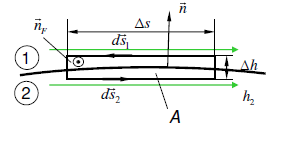
\includegraphics[width = 3.5cm]{./img/tang_rand.png}\end{center}
	\begin{emphbox}
		$\mathbf{n} \times (\mathbf{h}_1 - \mathbf{h}_2) = 
		\begin{cases}
				0 : \text{Normalfall} \\
			\mathbf{j}_F : \text{Oberflächenströme}
		\end{cases}$
	\end{emphbox}

\begin{emphbox}
	$\mathbf{n} \times (\mathbf{e}_1 -\mathbf{e}_2) = 0$\\
	Keine magnetischen Oberflächenströme
\end{emphbox}


\end{sectionbox}
\begin{sectionbox}
Normalenkomponente an einer Grenzschicht:\\
\vspace{-0.28cm}
\begin{center}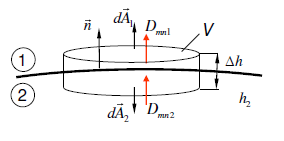
\includegraphics[width = 3.5cm]{./img/normal_rand.png}\end{center}
\begin{emphbox}
	$\mathbf{n} \cdot (\mathbf{D}_1 - \mathbf{D}_2) = \begin{cases}
		0 : \text{Normalfall} \\
		\rho_F: \text{Oberflächenladungen}
	\end{cases} $
\end{emphbox}

\begin{emphbox}
	$\mathbf{n} \cdot (\mathbf{b}_1 - \mathbf{b}_2) = 0$\\
	Keine magnetischen Oberflächenladungen
\end{emphbox}
\end{sectionbox}

\begin{sectionbox}
\subsection{Skin-Effekt}
Ansatz: $\nabla \times \mathbf{J} = -j\omega\kappa \mathbf{B}$, $\nabla\times\mathbf{B} = \mu \mathbf{J}$ und Strom in +z $\mathbf{J} = J_z \mathbf{u}_z$.\\
Es ergibt sich eine DGL: $\frac{\partial^2 J_z}{\partial y^2} = j\omega \mu \kappa J_z$
Im idealen elektrischen Leiter (PEC) $\kappa \to \infty: E_{tan} = 0$ an der Leiteroberfläche d.h.:\\
\begin{itemize}
	\item Der Leiter ist feldfrei! Kein elektrisches Feld im inneren des Leiters!
	\item nur an in einer infinitesimal dünnen Schicht existieren Oberflächenströme
\end{itemize}
Im schlechten Leiter d.h. $\kappa < \omega\epsilon$ breitet sich im Leiter eine gedämpfte Welle aus.\\
Im guten Leiter $\kappa >> \omega\epsilon$ gilt:
\begin{itemize}
	\item[1.] Das Feld fällt mit zunehmender Tiefe schnell ab
	\item[2.] In einer dünnen Schicht unter der Oberfläche existieren nennenswerte Stromdichten
	\item[3.] Für die Verluste sind also nur die obersten Schichten (die Haut) des Leiters entscheidend
\end{itemize}
Für die Stromverteilung im Leiter gilt: $J_z = J_z(0)\cdot e^{-ky}\cdot e^{-jky}$ mit $k = \sqrt{\frac{\omega\mu\kappa}{2}}\quad[\frac{1}{m}]$\\
Der Kehrwert der Abklingkonstante/Wellenzahl $k$ wird als Eindringtiefe bezeichnet. Das Amplitude der Stromdichte ist nach dieser Tiefe auf $1/e$ abgefallen.
\begin{emphbox}
Eindringtiefe: $\delta = \frac{1}{k} = \sqrt{\frac{2}{\omega \mu \kappa}}$
\end{emphbox}
Die Verluste im Material lassen sich berechnen (Platte mit Querschnitt $\delta \cdot a$)\\
\begin{tabular*}{\columnwidth}{ll}
	Oberflächenresistanz & $R_S = \frac{\omega\mu}{2\kappa} \quad [\Omega]$ \\
	Oberflächenimpedanz & $Z_S = R_S\cdot(1+j)$ \\
	Verluste durch Oberflächenströme & $P_J = \frac{1}{2} \iint R_S |H_0|^2 d\mathbf{A}$ \\
\end{tabular*}
\begin{tabular*}{\columnwidth}{ll}
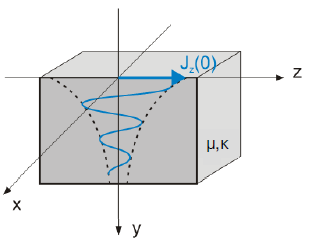
\includegraphics[width = 2.5cm]{./img/skin_effekt.png} & 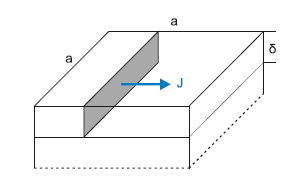
\includegraphics[width = 2.5cm]{./img/skin_effekt_verlust.png}\\
\end{tabular*}
\end{sectionbox}
\begin{sectionbox}
\subsubsection{Skin-Effekt Zusammenfassung}
\begin{itemize}
	\item Der Skin-Effekt stellt eine Näherung der Feldverteilung für gute Leiter dar. Diese Bedingung ist frequenzabhängig (auch wegen der Permittivität)
	\item Wichtige Voraussetzung: Verschiebeströme d.h. elektrische Flussdichte ist im Leiter vernachlässigbar.
	\item Bei hohen Frequenzen ist der Skin-Effekt nur in sehr guten Leitern anzunehmen, dann aber besonders ausgeprägt.
	\item Die Feldstärke und die Stromdichten fallen im Leiter exponentiell ab.
	\item Die Eindringtiefe sinkt jeweils mit der Quadratwurzel der Frequenz, der Leitfähigkeit und der Permeabilität.
	\item Die Eindringtiefe $\delta$ kennzeichnet den $1/e$-Abfall des Feldes. Der 10\% Abfall liegt bei etwa $2 \frac{1}{2} \delta$, der 1\%-Abfall bei etwa $4 \frac{1}{2} \delta$.
	\item Der Skin-Effekt basiert letztlich auf der elektromagnetischer Induktion (Ausgangspunkt der Herleitung)
\end{itemize}
\end{sectionbox}

\begin{sectionbox}
\subsection{Ebene Wellen}
Ausbreitungsgeschwindigkeit: $c = \frac{1}{\sqrt{\mu \cdot \epsilon}}$\\
Feldwellenwiderstand: $Z_F = \sqrt{\frac{\mu}{\epsilon}} = \sqrt{\frac{\mu_r}{\epsilon_r}}Z_{F_0}$\\
Feldwellenwiderstand im Freiraum: $Z_{F_0} = \sqrt{\frac{\mu_0}{\epsilon_0}} \approx 120\pi\Omega \approx 377\Omega$\\
Phasenkonstante: $\beta = \frac{\omega}{c} = \frac{2\pi}{\lambda}$\\

Lösungen für Wellengleichung:

\begin{tabular*}{\columnwidth}{l}
	$E_x(z) = E\cdot e^{-j\beta z}$ \\
	$H_y(z) = \frac{E}{Z_F} \cdot e^{-j\beta z}$\\
	$e_x(z,t) = Re\{ E_x(z) \cdot e^{j\omega t} \}$\\
	$e_x(z,t) = E_1 \cdot cos(\omega t - \beta z)$\\
	$e_y(z,t) = E_2 \cdot cos(\omega t - \beta z)$\\
\end{tabular*}

\subsubsection{Polarisation ebener Wellen}

\begin{center}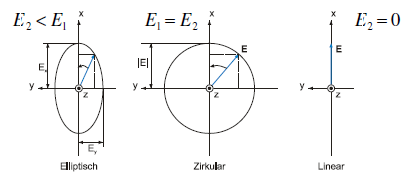
\includegraphics[width = 0.8\columnwidth]{./img/polarisation_ebener_wellen.png} \end{center}
\textbf{Eigenschaften ebene Wellen:}
\begin{itemize}
	\item Phasenfronten sind Ebenen, Wellenvektor ist Normalenvektor dieser Ebenen
	\item Gute Näherung für alle Wellen im Fernfeld
	\item Dispersionsfrei, TEM-Welle
	\item Zu jedem Wellenvektor existieren immer genau zwei unterscheidbare (orthogonale) Feldverteilungen ("Polarisation")
\end{itemize}

\textbf{Polarisation:}
\begin{itemize}
	\item Lineare Polarisation: Richtung des E-Feldvektors bleibt während der Ausbreitung konstant, seine Amplitude ändert sich sinusförmig, Polarisation wird nach dessen Richtung bezeichnet.
	\item Zirkulare Polarisation: Richtung des E-Feldvektors rotiert, seine Amplitude bleibt konstant, Polarisation wird nach Rotationsrichtung in Ausbreitungsrichtung bezeichnet.
\end{itemize}
	
\end{sectionbox}
\begin{sectionbox}
	\subsection{K-Raum Darstellung der MWG (quellfreier Fall)}
	Allgemeiner Ansatz: $\mathbf{E} = \mathbf{E}_0 \cdot e^{-j \mathbf{k}\cdot\mathbf{r}}$, $\mathbf{H} = \mathbf{H}_0 \cdot e^{-j \mathbf{k}\cdot\mathbf{r}}$\\
	Zeitlich: $e^{j\omega t}$, \quad $\mathbf{E}_0$,$\mathbf{H}_0$ konst.\\
	Wellenzahlvektor: $\mathbf{k} = k_x\mathbf{e}_x + k_y\mathbf{e}_y + k_z\mathbf{e}_z$\\
	Ortsvektor: $\mathbf{r} = r_x\mathbf{e}_x + r_y\mathbf{e}_y + r_z\mathbf{e}_z$\\
	Damit gilt: $\nabla = -j\mathbf{k} $\\
	
	Es ergibt für die Helmholtz Gleichung:\\
	$[\nabla^2 + \omega^2\epsilon\mu]\mathbf{E} = [-\mathbf{k}\cdot\mathbf{k} + \omega^2\epsilon\mu]\mathbf{E} = 0$\\
	$\mathbf{k}\cdot\mathbf{k} = \omega^2\epsilon\mu$ mit $j\mathbf{k} = \mathbf{\alpha} + j\mathbf{\beta}$\\
	
	\begin{emphbox}
		$\mathbf{k}\cdot\mathbf{k} = \mathbf{\beta}^2 - \mathbf{\alpha}^2 -j2\mathbf{\alpha}\cdot\mathbf{\beta} = \omega^2\epsilon\mu$
	\end{emphbox}
Verlustloste Medien: $\omega^2\epsilon\mu$ reell und $\mathbf{k}\cdot\mathbf{k} = \beta^2 - \alpha^2$.
\end{sectionbox}
\begin{sectionbox}
	\subsection{Fallunterscheidung für $\alpha$ und $\beta$}
	\textbf{1. Fall}: $\alpha = 0$, $\beta = \mathbf{k}$\\
	\begin{itemize}
		\item Ungedämpfte Welle mit Phasenkonstante $\beta$
		\item Verluste werden über komplexe Materialparamter berücksichtigt
		\item $\mathbf{E} = \mathbf{E}_0 e^{-j\mathbf{k}\cdot \mathbf{r}} $
		\item $\mathbf{H} = \frac{1}{Z_F}(\mathbf{e}_k \times \mathbf{E}_0) e^{-j\mathbf{k}\cdot \mathbf{r}} $
		\item $\mathbf{k} = k \mathbf{e}_k$, \quad $k=\omega\sqrt{\epsilon\mu}$
		\item Leistungstransport: $\mathbf{S} = \frac{\mathbf{e}_k}{2Z^*_F}  \mathbf{E} \cdot \mathbf{E} = \frac{\mathbf{e}_k Z^*_F}{2}\mathbf{H}\cdot\mathbf{H}^*$
		
	\end{itemize}
\textbf{2. Fall}: $\alpha \cdot \beta = 0$
\begin{itemize}
	\item Quergedämpfte Wellen (auch evaneszente Wellen)
	\item Phasenflächen eben
	\item Keine Dämpfung in Ausbreitungsrichtung $\beta$
	\item Amplituden auf Phasenflächen nicht konstant (in $\alpha$ Richtung gedämpft: keine Absorption)
\end{itemize}
\end{sectionbox}

\begin{sectionbox}
	\subsection{Reflexion und Brechung}
	\subsubsection{Senkrechter Einfall auf dielektrische Grenzfläche}
	
	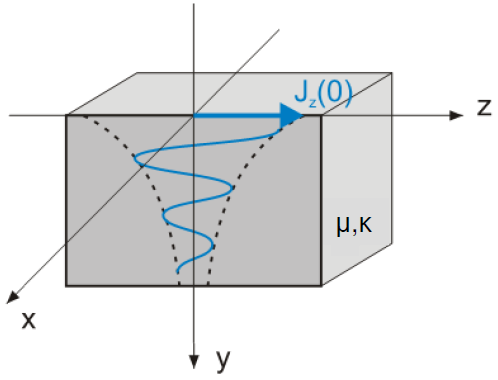
\includegraphics[width = 0.8\columnwidth]{./img/senkrecht_dielektrisch_einfall.png}
	
	\begin{tablebox}{@{\hspace{5mm}}c@{\extracolsep\fill}c@{\extracolsep\fill}}
	Reflexionsfaktor & Transmissionsfaktor \\
	$\rho = \frac{Z_{F2} - Z_{F1}}{Z_{F1} + Z_{F2}}$ & $\tau = \frac{2Z_{F2}}{Z_{F1} + Z_{F2}} = 1 + \rho$\\
	\end{tablebox}
	Welle in Medium 1: $\mathbf{E}_1(z) = E_{1i}e^{-j\beta_1z}(1+\rho e^{+2j\beta_1z})\mathbf{u}_x$\\
	Welle in Medium 2: $\mathbf{E}_2(z) = \tau E_{1i}e^{-j\beta_1z}\mathbf{u}_x$ \danger{Vorzeichen von $z$!}\\
	Stehwellenverhältnis: SWR = $\frac{|E_1|_{\text{max}}}{|E_1|_{\text{min}}} = \frac{1 + |\rho |}{1-|\rho |}$\\
	Max/Min: $z = -\frac{n \lambda_1}{2}, n= 0,1,2,\dots$, $|E_1| = |E_{1i}||1 + \rho|$\\
	Min/Max: $z = -\frac{(2n+1) \lambda_1}{4}, n= 0,1,2,\dots$, $|E_1| = |E_{1i}||1 - \rho|$\\
	Maximum/Minimum abhängig von ($\rho > 0$)/($\rho < 0$)\\
	Umformungen: $|\rho | = \frac{\text{SWR} - 1}{\text{SWR} + 1}$, $Z_{F2} = \frac{1 + \rho}{1 - \rho}Z_{F1}$ \\
	Vorzeichen: $\rho > 0$ für $Z_{F2} > Z_{F1}$ (falls reell)\\
	Leistungsfluss in 1: $|S| = \frac{|E_{1i}|^2}{Z_{F1}} - \frac{|E_{1r}|^2}{Z_{F1}} = \frac{|E_{1i}|^2}{Z_{F1}}(1 - \rho^2)$\\
\end{sectionbox}

\begin{sectionbox}
	\subsubsection{Schräger Einfall auf dielektrische Grenzfläche}
	Snelliussches Brechungsgesetz: $\frac{sin\theta_1}{sin\theta_2} = \frac{n_2}{n_1} = \sqrt{\frac{\epsilon_2\mu_2}{\epsilon_1\mu_1}}$\\
	\textbf{Brewster Winkel:} 
	Er gibt den Winkel an, bei dem nur die senkrecht zur Einfallsebene polarisierten Anteile (bezogen auf die elektrische Feldkomponente) reflektiert werden. Das reflektierte Licht ist dann linear polarisiert.\\
	$\theta_B = arctan(\frac{n_2}{n_1})$
	
	\begin{tablebox}{@{\hspace{5mm}}c@{\extracolsep\fill}|c@{\extracolsep\fill}}
		Reflexionsfaktor & Transmissionsfaktor \\
		\hline\\
		$\rho_{\perp} = \frac{Z_{F2}cos\theta_1 -Z_{F1}cos\theta_2}{Z_{F2}cos\theta_1 + Z_{F1}cos\theta_2}$ & $\tau_{\perp} = \frac{2Z_{F2}cos\theta_1}{Z_{F2}cos\theta_1 + Z_{F1}cos\theta_2}$ \\
		\\
		$\rho_{\parallel} = \frac{Z_{F1}cos\theta_1 -Z_{F2}cos\theta_2}{Z_{F2}cos\theta_1 + Z_{F1}cos\theta_2}$ & $\tau_{\parallel} = \frac{2Z_{F2}cos\theta_1}{Z_{F1}cos\theta_1 + Z_{F2}cos\theta_2}$
	\end{tablebox}
\end{sectionbox}

\begin{sectionbox}
	\begin{tabular*}{\columnwidth}{cc}
	Senkrechte Polarisation & Parallele Polarisation \\
	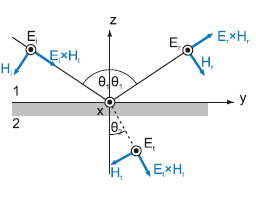
\includegraphics[width = 3.1cm]{./img/fresnel_perp.png} & 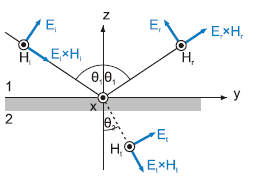
\includegraphics[width = 3.1cm]{./img/fresnel_parallel.png}
\end{tabular*}

\end{sectionbox}

\begin{sectionbox}
	\subsubsection{Schräger Einfall auf leitende Grenzfläche}
	\textbf{1. Fall: Senkrechte Polarisation}\\
	$\mathbf{E}_i(y,z) = Ee^{-j\beta (y\sin{\theta} - z\cos{\theta} )}\mathbf{u}_x$\\
	$\mathbf{E}_r(y,z) = Ee^{-j\beta (y\sin{\theta} + z\cos{\theta} )}\mathbf{u}_x$\\
	$\Rightarrow$ stehende Welle in z-Richtung und eine Wanderwelle in y-Richtung:\\
	$\mathbf{E}_{\text{tot}}(y,z) = 2jE\sin{(\beta\cos{\theta} z )}e^{-j \beta\sin{\theta} y }\mathbf{u}_x$\\
	\textbf{2. Fall: Parallele Polarisation}\\
	Parallel zur Ebene:\\
	$E_{i y}(y,z) = E \cos{\theta}e^{-j\beta(y\sin{\theta}-z\cos{\theta})}$\\
	$E_{r y}(y, z)=-E \cos \theta e^{-j \beta(y \sin \theta+z \cos \theta)}$\\
	Senkrecht zur Ebene:\\
	$E_{i z}(y, z)=E \sin \theta e^{-j \beta(y \sin \theta-z \cos \theta)}$\\
	$E_{r z}(y, z)=E \sin \theta e^{-j \beta(y \sin \theta+z \cos \theta)}$\\
	$\Rightarrow$ stehende Welle in z-Richtung und eine Wanderwelle in y-Richtung:\\
	$E_{\text {tot } y}(y, z)=2 j E \cos \theta \sin (\beta z \cos \theta) e^{-j \beta y \sin \theta}$ \\
	$E_{\text {tot } z}(y, z)=2 E \sin \theta \cos (\beta z \cos \theta) e^{-j \beta y \sin \theta}$
\end{sectionbox}

\begin{sectionbox}
	\subsection{Zusammenfassung Reflexion, Transmission an Grenzflächen}
	\begin{itemize}
		\item Die Reflexion (und Transmission) einer ebenen Welle an einer senkrecht zur Ausbreitungsrichtung orientierten Grenzfläche folgt den gleichen Gesetzmäßigkeiten wie bei einer (fehl-)abgeschlossenen TEM-Leitung. Dabei gilt:
		\subitem Leitende Wand: Kurzschluss
		\subitem Magnetische Wand: Leerlauf
		\subitem Dielektrische Wand: Leitung mit anderem Wellenwiderstand
		\item Die Reflexion (und Transmission) einer ebenen Welle an einer schräg zur Ausbreitungsrichtung orientierten Grenzfläche lässt sich als Überlagerung zweier Wellen beschreiben:
		\item Die jeweiligen Teilwellen ergeben sich als Projektion des Wellenvektors auf (1) den Normalenvektor und (2) die Oberfläche der Grenzfläche
		\item Für die erste Teilwelle gelten die Reflexions- und Transmissionseigenschaften einer Welle bei senkrechtem Einfall
		\item Die zweite Teilwelle ist eine reflexionsfreie "Oberflächenwelle" entlang der Grenzfläche
	\end{itemize}
\end{sectionbox}
\begin{sectionbox}
	\subsection{Gauß'scher Strahl}
	\begin{emphbox}
		$E(x,y,z) = E_0\frac{w_0}{w(z)}exp\left(-\frac{x^2+y^2}{w(z)^2} -jkz - \frac{j\pi (x^2+y^2)}{\lambda R(z)} +j\text{arctan}\frac{\lambda z}{\pi \omega_0^2}\right)$
	\end{emphbox}
	\begin{itemize}
		\item $E_0 = \sqrt{\frac{4 k_{0} Z_{F 0} P}{\pi b}}$, mit $k_0 = \frac{2\pi f}{c}$ (ungedämpft)
		\item $b = n k_0 w_0^2[m]$, mit Brechzahl $n = \sqrt{\epsilon_r \mu_r}$, \danger{!$w_0$ ist nicht $\omega_0$}
		\item Strahldurchmesser (Abfall auf 1/e): $w(z) = w_0 \sqrt{1 + \left(\frac{2z}{b}\right)^2}$
		\item Amplitudenterm: $-\frac{x^2+y^2}{w(z)^2}$
		\item Phasenterm: $-jkz$
		\item Krümmung der Phasenfronten: $- \frac{j\pi (x^2+y^2)}{\lambda R(z)}$
		\item Korrekturfaktor (damits aufgeht): $+j\text{arctan}\frac{\lambda z}{\pi \omega_0^2}$
	\end{itemize}
	Für große Werte von $|z|$ schmiegt sich das Hyperboloid asymptotisch einem Kegel an mit dem Öffnungswinkel:\\
	$\theta_0 = \text{arctan}\frac{2w_0}{b}$\\
	$w(z) = z\tan\theta$\\
	Für $z \gg b$: $\frac{w_0}{w(z)} \approx \frac{b}{2z}$
	
	Für kleine Öffnungswinkel erhalten wir näherungsweise:\\
	$\theta_0 = \frac{\lambda}{\pi w_0} = \frac{2w_0}{b} = \frac{2}{nk_0w_0} = \frac{\lambda_0}{\pi w_0 n}$\\
	$b=\frac{2 \lambda}{\pi \theta_{0}^{2}}$

	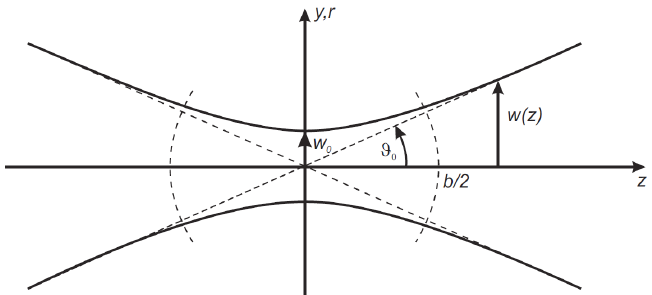
\includegraphics[width = \columnwidth]{./img/gauss_strahl.png}\\
	
	Leistungstransport des Strahls:\\
	$P = \frac{n}{2Z_{F0}}\int_-\infty^\infty\int_-\infty^\infty |E_{00x}(x,y,z)|^2 dxdy$

	Konfokaler Parameter $b$:\\
	Im konfocalen Abstand $z=\pm b/2$ ist die doppelte Fläche beschienen: $w(z) = \sqrt{2}w_0$.
\end{sectionbox}
\section{Leitungen}
\begin{sectionbox}
\subsection{Telegraphengleichungen}
Aus dem Ersatzschaltbild für die verlustlose Leitung $R'=G'=0$ bzw $R'<< \omega L'$ und $G' << \omega C'$ werden die Telegraphengleichungen über KCL und KVL abgeleitet.

\begin{emphbox}
Spannung:\qquad	$\frac{\partial^2 u(t,z)}{\partial t^2} - \frac{1}{L' C'} \frac{\partial^2 u(t,z)}{\partial z^2} = 0$\\
Strom:	\qquad $\frac{\partial^2 i(t,z)}{\partial t^2} - \frac{1}{L' C'} \frac{\partial^2 i(t,z)}{\partial z^2} = 0$\\
\end{emphbox}
Ausbreitungsgeschwindigkeit: $c=\frac{1}{\sqrt{L' C'}}$\\
Das Verhältnis $c/c_0$ wird als Verkürzungsfaktor bezeichnet.\\
Typisch: $\frac{c}{c_0} \approx 0.66$ bzw. $c\approx 2 \cdot 10^8 [\frac{m}{s}]$\\

\end{sectionbox}

\begin{sectionbox}
	\subsection{Ersatzschaltbild Leitung und wichtige Parameter}
	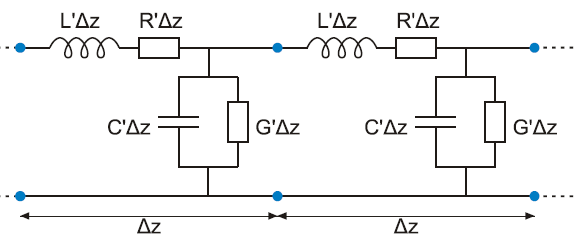
\includegraphics[width = \columnwidth]{./img/ersatzschaltbild_leitung.png}\\
	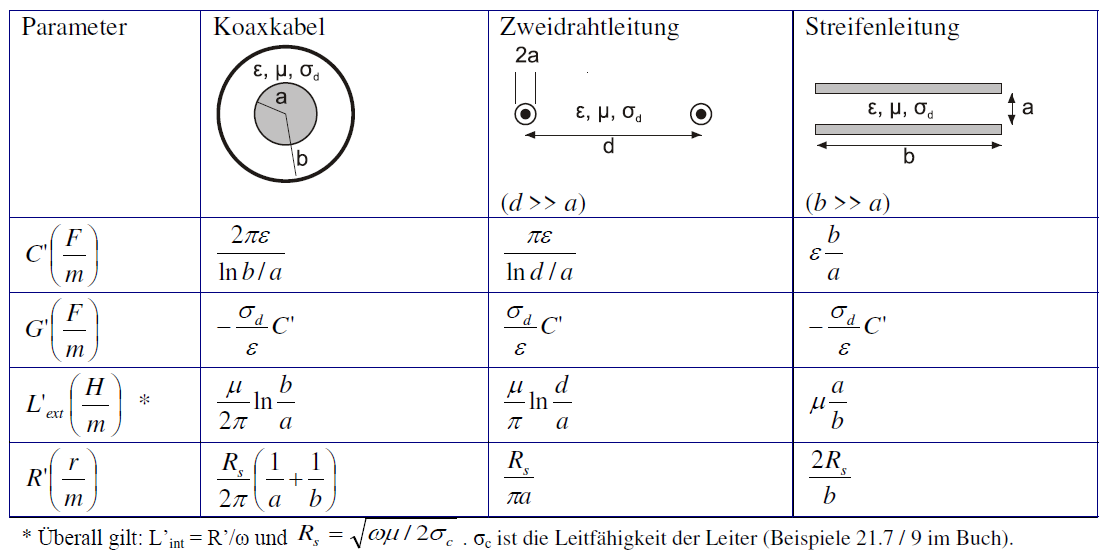
\includegraphics[width = \columnwidth]{./img/parameter_leitungen.png}\\
\end{sectionbox}
\begin{sectionbox}
	\subsection{Lösung der Telegraphengleichungen}
	Ansatz: $u,i \propto e^{j\omega t}$. Damit werden werden die zeitlichen Ableitungen wieder zu $j\omega$\\
	
	Spannung:\qquad $V(z) = V_+ e^{-j\beta z} + V_- e^{+j\beta z}$\\
	Strom:	\qquad$I(z) = \frac{V_+}{Z_0} e^{-j\beta z} - \frac{V_-}{Z_0} e^{+j\beta z}$\\
	Phasenkonstante: $\beta = \omega\sqrt{L' C'} = \frac{\omega}{c}$, $\lambda = \frac{c}{f} = \frac{2\pi}{\beta}$\\
	Charakteristische Impedanz: $Z_0 = \sqrt{\frac{L'}{C'}}$
	
\end{sectionbox}
\begin{sectionbox}
	\subsection{Zusammenfassung Leitungen}
	\begin{itemize}
	\item Die ideale TEM-Leitung kann vollständig netzwerktheoretisch beschrieben werden. Es handelt sich dabei nicht um Wellenausbreitung im eigentlichen Sinne
	\item Die Netzwerkgrößen I(t,z) und V(t,z) stehen aber in einer räumlichen und zeitlichen Beziehung, gekennzeichnet durch die Ausbreitungsgeschwindigkeit, die unabhängig von der Signalform ist.
	\item Dabei existieren immer zwei unabhängige Lösungen, die den beiden möglichen Transportrichtungen entsprechen.
	\item Die Leitungseigenschaften $c$ und $Z_0$ sind für beide Lösungen und an allen Orten der Leitung gleich und ausschließlich durch die Leitungsgeometrie und die Materialien festgelegt.
	\item Die Ausbreitungsgeschwindigkeit ist nur dann kleiner als $c_0$, wenn das elektrische und/oder magnetische Feld der Leitung dielektrische und/oder magnetisches Material durchdringt.
	\item Sämtliche Leitungseigenschaften lassen sich durch eine (quasi-)statische Analyse ermitteln ($C'$ und $L'$ sind auch für Gleichstrom definiert).
	\end{itemize}
\end{sectionbox}

\begin{sectionbox}
	\subsection{Abschluss einer Leitung}
	Ist der Abschluss der Leitung fehlt angepasst entsteht eine reflektierte Welle. Der Reflexionsfaktor ist das Verhältnis aus zurücklaufender Welle zu einfallender Welle.\\
	\textbf{Reflexionsfaktor}: \quad $\rho(0) = \frac{V_-(0)}{V_+(0)}$\\
	
	\begin{tablebox}{@{\hspace{5mm}}l@{\extracolsep\fill}|l@{\extracolsep\fill}}
		Kurzschluss & $V=0,\implies V_+ = -V_- \implies \rho=\frac{V_-}{-V_-} = -1$ \\
		\hline
		Leerlauf & $I=0,\implies V_+ = V_-, \implies V=2V_+, \quad \rho=+1$\\
		\hline
		Reflexionsfrei & $V_- = 0, \implies V=V_+,\implies \quad \rho=0$ 
	\end{tablebox}
Im Lastwiderstand umgesetzte Leistung: $P_L = \frac{|V_+|^2}{Z_0}(1-|\rho|^2)$
\end{sectionbox}

\begin{sectionbox}
	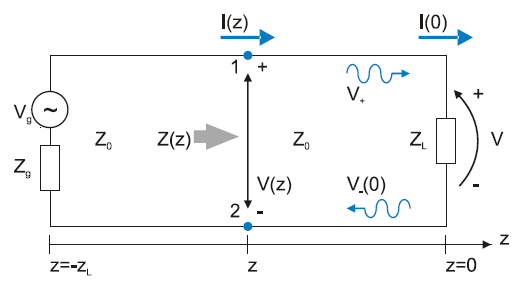
\includegraphics[width = \columnwidth]{./img/reflexion_leitung.png}\\
\end{sectionbox}
\begin{sectionbox}
	\subsection{Zusammenhang Reflexionsfaktor und Leitungsimpedanz}
	
	Bei der Impedanz $Z(\xi)$ liegt der Ursprung in der Last wird aber nach links und
	nicht nach rechts positiv gemessen d.h.: $\xi = -z$\\
	
	$\rho = \frac{Z_L - Z_0}{Z_L + Z_0}$ \quad
	$Z(\xi) = Z_0 \frac{1+\rho e^{-j2\beta\xi}}{1-\rho e^{-j2\beta\xi}}$\\
	
		\begin{tablebox}{@{\hspace{5mm}}l@{\extracolsep\fill}|l@{\extracolsep\fill}}
		Leerlauf & $Z_L \to \infty, \frac{Z(xi)}{Z_0} = -jcot\beta\xi$, f. $\xi <\frac{\lambda}{4}$:kapazitiv\\
		\hline
		Kurzschluss & $Z_L = 0, \frac{Z(\xi)}{Z_0} = jtan\beta\xi$, f. $\xi<\frac{\lambda}{4}$: induktiv\\
		\hline
		$\frac{\lambda}{4}$ Trans. & $\beta z = \pi/2$ d.h. $tan(\beta z) \to \infty$\\
	\end{tablebox}

	$\frac{\lambda}{4}$ Transformator: $\frac{Z\left(\frac{\lambda}{4}\right)}{Z_0} = \frac{Z_0}{Z_L}$\\
	
	\textbf{Anpassleitung}: $Z_0 = \sqrt{Z(\lambda /4)\cdot Z_L}$\\
	\textbf{Stehwellenverhältnis}: $\text{VSWR} =\frac{V_{max}}{V_{min}} = \frac{1+|\rho |}{1- |\rho |}$\\
	$V_{max}$ und $V_{min}$ an der Last gemessen.	
\end{sectionbox}
\begin{sectionbox}
	\subsection{Verlustbehaftete Leitung}
	$Z_0 = \sqrt{\frac{R' +j\omega L'}{G' + j\omega C'}}$\\
	\textbf{Komplexe Ausbreitungskonstante}:\\
	
	$\gamma = \alpha + j\beta = \sqrt{(R' + j\omega L')(G'+j\omega C')}$\\
	Im üblichen Fall $R' << \omega L'$, $G' << \omega C'$ erhält man:\\
	
	$\alpha \approx \frac{1}{2}\left(R'\sqrt{\frac{C'}{L'}} + G'\sqrt{\frac{L'}{C'}} \right)$\\
	$G' \to 0$: $\alpha \approx \frac{1}{2} \frac{R'}{Z_0}$, $\beta \approx \omega\sqrt{L'C'}$\\
	
	\begin{itemize}
		\item Ein Leitungsstück der Länge $d$ weist dann die Dämpfung: $\frac{V_2}{V_1}=e^{-\alpha d}$ auf
		\item $ln(e^{-\alpha d}) = -\alpha d \quad[\text{Np}]$
		\item $20log(e^{-\alpha d}) = -20log(e)\alpha d \quad [\text{dB}]$
		\item 1Np = $8.685$dB
	\end{itemize}
\end{sectionbox}
\begin{sectionbox}
	\subsection{Transformation ins Smith-Diagramm}
	Mit einer konformen Abbildung können Reflexionsfaktor und Leitungsimpedanz ineinander überführt werden.\\
	
	$z=\frac{Z_L}{Z_0} \text{dann} \quad \begin{cases}
		\rho = \frac{z-1}{z+1}\\
		z = \frac{1+\rho}{1-\rho}
	\end{cases}$
\end{sectionbox}

\begin{sectionbox}
	\subsection{Regeln Smith-Chart}
	\begin{itemize}
		\item Die horizontale Achse entspricht reellen Widerständen bzw. Leitwerten
		\item Der \textbf{Kurzschlusspunkt} liegt \textbf{links}, der \textbf{Leerlauf} \textbf{rechts}
		\item Die Punkte auf dem Umfang entsprechen rein imaginären $z$ bzw $y$.
		\item Der \textbf{Mittelpunkt} ist der \textbf{Anpasspunkt}.
		\item Kreise um Mittelpunkte auf der horizontalen Achse (rechts von "M") entsprechen Widerständen mit konstantem Realteil
		\item Kreise um Mittelpunkte auf der Senkrechen durch $O$ entsprechen Widerständen mit konstantem Imaginärteil
		\item Kreise um Mittelpunkte auf der horizontalen Achse (links von "M") entsprechen Leitwerten mit konstantem Realteil.
		\item Kreise um Mittelpunkte auf der Senkrechten durch "S" entsprechen Leitwerten mit konstantem Imaginärteil
		\item Die obere Hälfte des Diagramms entspricht induktiven Reaktanzen bzw. kapazitiven Suszeptanzen
		\item Die untere Hälfte des Diagramms entspricht kapazitiven Reaktanzen bzw. induktiven Suszeptanzen
		\item Kreise um den Mittelpunkt entsprechen Leitungstransformationen in verlustlosen Leitungen: Bewegt man sich vom Abschlusswiderstand weg (Vergrößerung der Leitungslänge), dann bewegt man sich im Uhrzeigersinn.
	\end{itemize}
\end{sectionbox}

\begin{sectionbox}
	\subsection{Planare Leitungen}
	\begin{tabular*}{\columnwidth}{cc}
		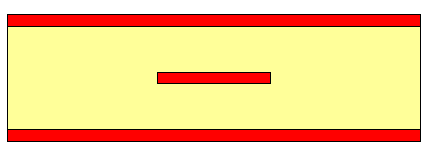
\includegraphics[width = 3cm]{./img/streifenleitung.png} & 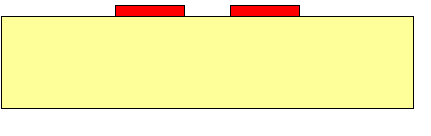
\includegraphics[width = 3cm]{./img/koplanar_streifen_leitung.png}\\
		Streifenleitung & Koplanare Streifenleitung\\
		\hline\\
		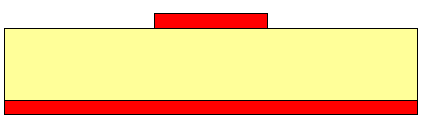
\includegraphics[width = 3cm]{./img/mikrostreifen_leitung.png} & 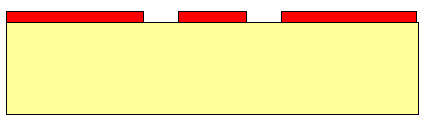
\includegraphics[width = 3cm]{./img/koplanar_leitung.png}\\
		Mikrostreifenleitung & Koplanarleitung\\
	\end{tabular*}
	\vspace{-6mm}
	\begin{multicols*}{2}
	\begin{itemize}
		\item[+] einfache Fertigung
		\item[+] verlustarm
		\item[+] umepfindlich gg. Diskontinuitäten
		\item[+] Serienelemente leicht integrierbar
		\item[-] Parallelelemente schwierig
		\item[-] Leiterbreite nicht skalierbar
		\item[-] messtechnisch schwierig
	\end{itemize}
	\columnbreak
	\begin{itemize}
		\item[+] einseitige Metallisierung
		\item[+] Leiterbreite skalierbar
		\item[+] Serienelemente leicht integrierbar
		\item[+] Serienelemente leicht integrierbar
		\item[+] Parallelelemente leicht integrierbar
		\item[-] mittlere Verluste
		\item[-] zwei Moden $\rightarrow$ Leiterbrücken 
		\item[-] empfindlich gg. Diskontinuitäten 
	\end{itemize}
\end{multicols*}

Die einzige planare Leitung auf der eine TEM-Welle natürlich ausbreitungsfähig ist ist die Streifenleitung

\end{sectionbox}

\section{Zwei- und Mehrtore}
\begin{sectionbox}
Bei höheren Frequenzen sind bei Zwei- und Mehrtoren die Zuleitungen zu berücksichtigen. Daher ist die Definition der Bezugsebenen (Tor 1 und Tor 2) erforderlich.\\
Die Verwendung von Strom ($I_1$ bzw. $I_2$) und Spannung ($V_1$ und $V_2$) als Torgrößen ist wenig sinnvoll. Betrag und Phase hängen empfindlich von der Länge der Zuleitung ab.
Bei höheren Frequenzen werden fast ausschließlich komplexe Amplituden der hineinlaufenden Wellen ($a_1$ bw. $a_2$) und der herauslaufenden Wellen ($b_1$ bzw. $b_2$) als Torgrößen verwendet. Amplituden auf den Zuleitungen konstant, lediglich Phasenänderung.
\end{sectionbox}
\begin{sectionbox}
	\subsection{Komplexe Wellenamplituden}
	Spannung der hineinlaufenden Wellen:\\
	$V_{+i}e^{-j\beta z_i} = \frac{1}{2}(V_i(z_i) + Z_0 \cdot I_i(z_i))\cdot $\\
	Definition der Wellenamplituden über die Leistung:\\
	$P_{el} = \frac{1}{2}V\cdot V_{+i} \cdot I_{+i}^* = \frac{1}{2}V_{+i}\cdot \frac{V_{+i}^*}{Z_0} = \frac{V_{+i}}{\sqrt{2} Z_0}\cdot\frac{V_{+i}^*}{\sqrt{2} Z_0}$\\
	
	$P_{el} = a_i(z_i)\cdot a_i^*(z_i) = |a_i(z_i)|^2$
	Analog für herauslaufende Welle, es ergibt sich:\\
	$a_i(z_i) = \frac{V_{+i}\cdot e^{-j\beta z_i}}{\sqrt{2}Z_0}$, \qquad $[a_i] = \sqrt{\text{W}}$\\
	
	$b_i(z_i) = \frac{V_{-i}\cdot e^{-j\beta z_i}}{\sqrt{2}Z_0}$, \qquad $[b_i] = \sqrt{\text{W}}$\\
	
	$V_i(z_i) = \sqrt{2Z_0} \cdot (a_i(z_i) + b_i(z_i))$\\
	$I_i(z_i) = \frac{2}{Z_0} \cdot (a_i(z_i) - b_i(z_i))$
	
	Definition über Klemmspannungen und -ströme: (Ströme hineinlaufend)\\
	$a_{k}=\frac{1}{2 \sqrt{2 Z_{0}}}\left(U_{k}+Z_{0} \cdot I_{k}\right)$\\
	$b_{k}=\frac{1}{2 \sqrt{2 Z_{0}}}\left(U_{k}-Z_{0} \cdot I_{k}\right)$
\end{sectionbox}

\begin{sectionbox}
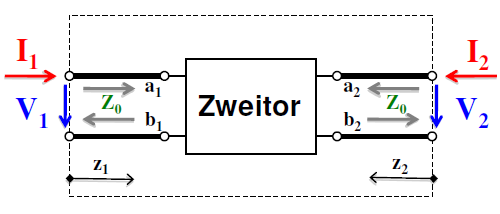
\includegraphics[width = \columnwidth]{./img/zweitor_amplituden.png}
\end{sectionbox}
\begin{sectionbox}
	\subsection{Streuparameter (S-Parameter)}
	$b_1 = S_{11} a_1 + S_{12} a_2$\\
	$b_2 = S_{21} a_1 + S_{22} a_2$\\
	\textbf{Matrizendarstellung}:\\
	$\begin{bmatrix}
		b_1 \\
		b_2
	\end{bmatrix}
	= [S] \begin{bmatrix}
		a_1\\
		a_2
	\end{bmatrix}$

	\textbf{Zusammenhang mit Reflexionsfaktor}:\\
	\begin{emphbox}
	Eingangsreflexionsfaktor: $\rho_E = \frac{b_1}{a_1} = S_{11} + \frac{S_{12}S_{21}\rho_L}{1-S_{22}\rho_L}$
	\end{emphbox}

	$\rho_L = \frac{a_2}{b_2}  \implies \frac{1}{\rho_L} = S_{22} + \frac{a_1}{a_2}\cdot S_{21}$\\
	
	$\rho_A = \frac{b_2}{a_2}, \quad \rho_G = \frac{a_1}{b_1}$\\
	\begin{emphbox}
		Ausgangsreflexionsfaktor: $\rho_A = S_{22} + \frac{S_{12}S_{21}\rho_G}{1-S_{11}\rho_G}$
	\end{emphbox}
Falls Zweitor rückwirkungsfrei: $S_{12} = 0 \implies \rho_E = S_{11}, \quad \rho_A = S_{22}$\\

\begin{tabular*}{\columnwidth}{cc}
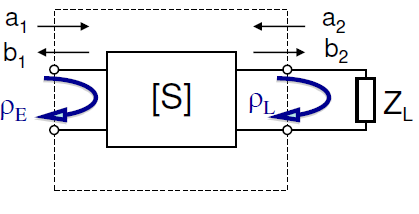
\includegraphics[width = 3cm]{./img/eingangsrefl.png} & 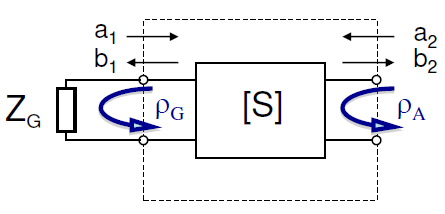
\includegraphics[width = 3cm]{./img/ausgangsrefl.png}
\end{tabular*}
\end{sectionbox}

\begin{sectionbox}
	\subsection{Stabilität von Zweitoren}
	Absolute Stabilität: Die Tore verhalten sich unabhängig von der Beschaltung passiv d.h. $Re\{Z_E\} > 0$ und $Re\{Z_A\} > 0$.\\
	Für die Reflexionsfaktoren muss gelten:\\
	\begin{emphbox}
		$|\rho_E < 1$ und $|\rho_A| < 1$ für\\
		
		$|\rho_L| < 1$ und $|\rho_G| < 1$
	\end{emphbox}
\end{sectionbox}


% \begin{sectionbox}
% 	\subsection{Besondere Zweitore}
% 	\setlength\tabcolsep{1.5pt}\begin{tabular*}{\columnwidth}{cc}
% 		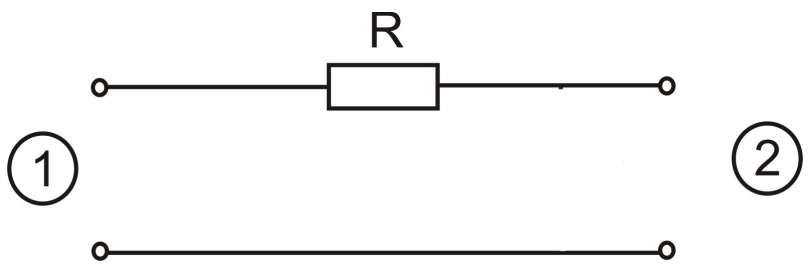
\includegraphics[width = 2.5cm]{./img/laengs_widerstand.png} & 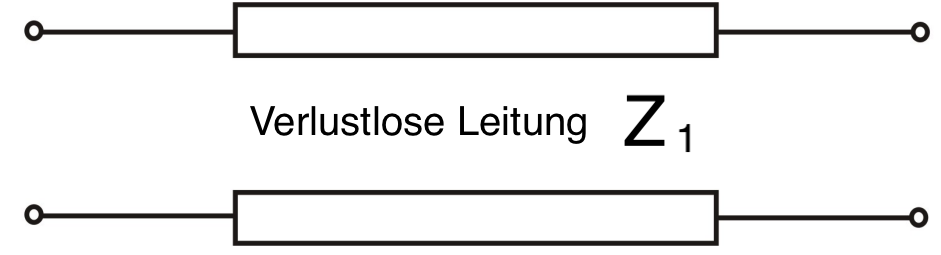
\includegraphics[width = 3cm]{./img/leitung.png}\\
% 		Längswiderstand & Verlustfreie Leitung\\
% 		$[S]=\left[\begin{array}{cc}
% 			\frac{R}{R+2 Z_{0}} & \frac{2 Z_{0}}{R+2 Z_{0}} \\
% 			\frac{2 Z_{0}}{R+2 Z_{0}} & \frac{R}{R+2 Z_{0}}
% 			\end{array}\right]$ & $U_{1}=U_{2} \cos (\beta l)+j Z_{L} I_{2} \sin (\beta l)$\\
% 		& $I_{1}=j \frac{U_{2}}{Z_{L}} \sin (\beta l)+I_{2} \cos (\beta l)$\\
% 	\end{tabular*}
% \end{sectionbox}

\begin{sectionbox}
	\subsection{Anpassung, Reziprozität, Symmetrie, Verlustfreiheit}
	\begin{emphbox}
		Anpassung: $S_{ii} = 0 \forall i$\\
		Reziprozität: $[S] = [S]^T$ ($[Y] = [Y]^T$)\\
		Symmetrie: $[S] = [S]^T$ und $S_{ii} = S_{jj} \forall i,j$\\
		Verlustfreiheit: $[S]^T[S]^* = [E]$
	\end{emphbox}
	Verlustfreiheit erfordert, dass die Betragsquadrate der Spalten $1$ ergeben.\\
	\textbf{Verlustfreies, reziprokes allseits angepasstes 3-Tor nicht realisierbar.}
\end{sectionbox}


\begin{sectionbox}
	\subsection{Alternative Netzwerkdarstellungen}
	\textbf{Transmissionsmatrix}:\\
	\setlength\tabcolsep{1.5pt}\begin{tabular*}{\columnwidth}{cc}
	$\left[\begin{array}{l}
		b_{1} \\
		a_{1}
		\end{array}\right]=[\Sigma]\left[\begin{array}{l}
		a_{2} \\
		b_{2}
		\end{array}\right]$ & \raisebox{-7mm}{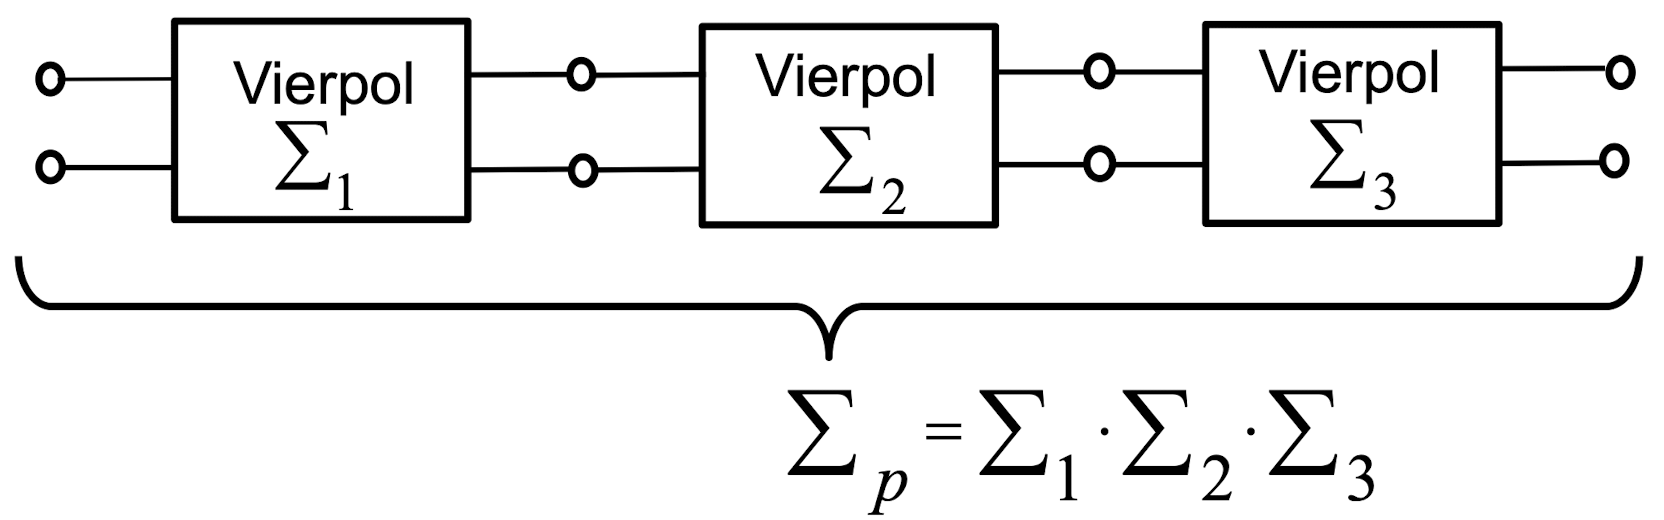
\includegraphics[width = 4cm]{./img/transmissions_matrix.png}}\\
	\end{tabular*}
	$[\Sigma]=\frac{1}{S_{21}}\left[\begin{array}{cc}
		-\Delta_{S} & S_{11} \\
		-S_{22} & 1
		\end{array}\right]$ $[S]=\frac{1}{\Sigma_{22}}\left[\begin{array}{cc}
			\Sigma_{12} & \Delta \Sigma \\
			1 & -\Sigma_{21}
			\end{array}\right]$\\
	Determinante: $\Delta A = A_{11}A_{22}-A_{12}A_{21}$\\

	\textbf{Kettenmatrix}:\\
	\setlength\tabcolsep{1.5pt}\begin{tabular*}{\columnwidth}{cc}
		$\left[\begin{array}{l}
			u_{1} \\
			i_{1}
			\end{array}\right]=\left[\begin{array}{ll}
			\mathrm{A} & \mathrm{B} \\
			\mathrm{C} & \mathrm{D}
			\end{array}\right]\left[\begin{array}{l}
			u_{2} \\
			-i_{2}
			\end{array}\right]$ & \raisebox{-4mm}{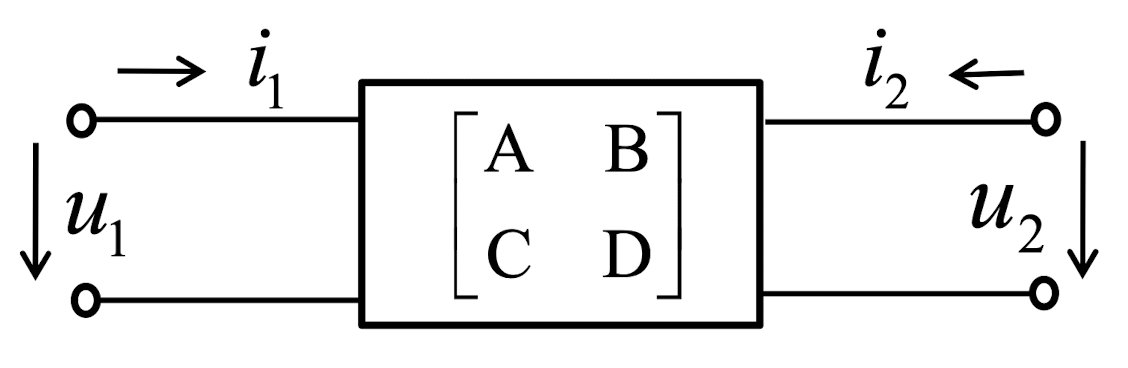
\includegraphics[width = 3cm]{./img/kettenmatrix.png}}\\
		\end{tabular*}\\

		Mit normierten Größen $u$,$i$ $[\sqrt{W}]$:\\
		$u = U / \sqrt{Z_0}$ und $i = I\sqrt{Z_0}$\\
		$u_{1,2}=a_{1,2}+b_{1,2}$, $i_{1,2}=a_{1,2}-b_{1,2}$\\
		\begin{tablebox}{@{\hspace{5mm}\vspace{1mm}}l@{\extracolsep\fill}l@{\extracolsep\fill}}
			$S_{11}=\frac{A+B-C-D}{A+B+C+D}$ & $S_{12}=\frac{2 \Delta_{A}}{A+B+C+D}$\\
			$S_{21}=\frac{2}{A+B+C+D}$ & $S_{22}=\frac{-A+B-C+D}{A+B+C+D}$\\
			\hline
			$A=\frac{-\Delta_{S}+S_{11}-S_{22}+1}{2 S_{21}}$ & $B=\frac{\Delta_{S}+S_{11}+S_{22}+1}{2 S_{21}}$\\
			$C=\frac{\Delta_{S}-S_{11}-S_{22}+1}{2 S_{21}}$ & $D=\frac{-\Delta_{S}-S_{11}+S_{22}+1}{2 S_{21}}$\\
		\end{tablebox}
\end{sectionbox}

\begin{sectionbox}
	\subsection{Kettenmatrizen häufiger 2-Tore}
	$\left[\begin{array}{cc}
		\mathrm{A} & \mathrm{B} \\
		\mathrm{C} & \mathrm{D}
		\end{array}\right]=\left[\begin{array}{cc}
		1 & \frac{R}{Z_{0}} \\
		0 & 1
		\end{array}\right]$ \raisebox{-4mm}{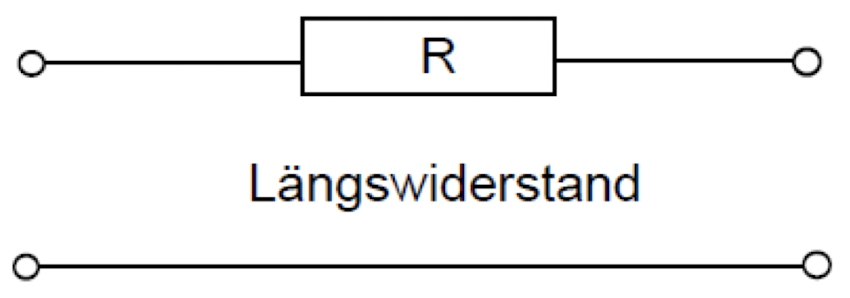
\includegraphics[width = 3cm]{./img/laengswiderstand.png}}\\
		$\left[\begin{array}{cc}
			\mathrm{A} & \mathrm{B} \\
			\mathrm{C} & \mathrm{D}
			\end{array}\right]=\left[\begin{array}{cc}
			1 & 0 \\
			G Z_{0} & 1
			\end{array}\right]$\raisebox{-4mm}{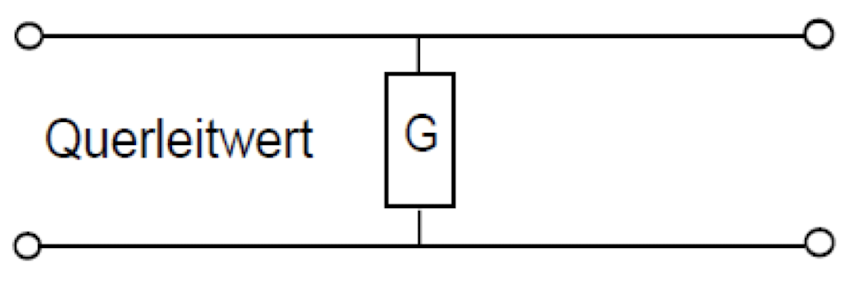
\includegraphics[width = 3cm]{./img/querleitwert.png}}\\
		$\left[\begin{array}{cc}
			\cos \beta l & j \frac{Z_{1}}{Z_{0}} \sin \beta l \\
			j \frac{Z_{0}}{Z_{1}} \sin \beta l & \cos \beta l
			\end{array}\right]$\raisebox{-4mm}{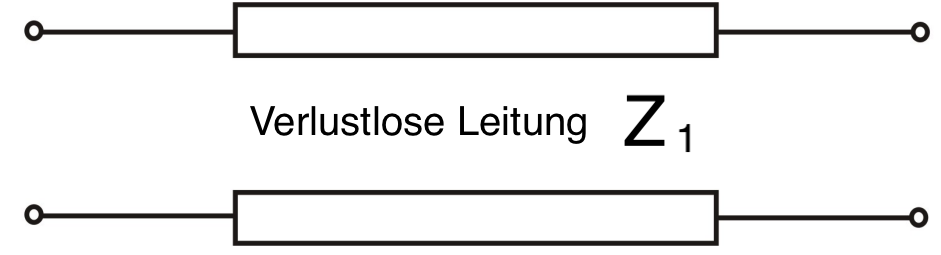
\includegraphics[width = 3cm]{./img/leitung.png}}\\
		$\left[\begin{array}{cc}
			\cosh \gamma l & \frac{Z_{1}}{Z_{0}} \sinh \gamma l \\
			\frac{Z_{1}}{Z_{0}} \sinh \gamma l & \cosh \gamma l
			\end{array}\right]$ \raisebox{-4mm}{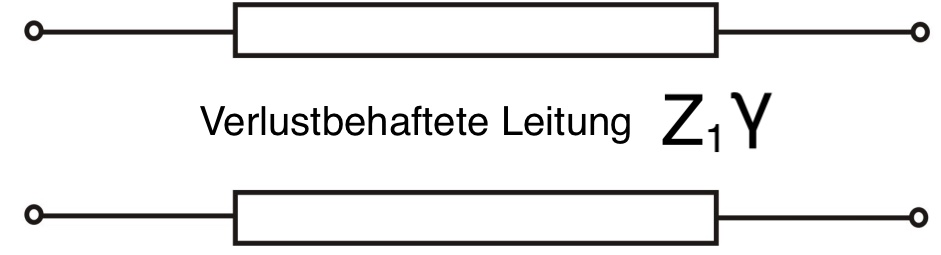
\includegraphics[width = 3cm]{./img/leitung_verlustbehaftet.jpg}}\\
		$\left[\begin{array}{ll}
			\mathrm{A} & \mathrm{B} \\
			\mathrm{C} & \mathrm{D}
			\end{array}\right]=\left[\begin{array}{cc}
			\frac{1}{n} & 0 \\
			0 & n
			\end{array}\right]$ Idealer Übertrager, $n = N_1 / N_2$\\
\end{sectionbox}
\begin{sectionbox}
	\subsection{Eingangswiderstände unter veschiedenen Anschlüssen}	
	\begin{tablebox}{@{\hspace{15mm}}l@{\extracolsep\fill}l@{\hspace{15mm}\extracolsep\fill}}
		Abschluss $Z_0$: & $Z_{i n}=\frac{\mathrm{A}+\mathrm{B}}{\mathrm{C}+\mathrm{D}} Z_{0}$\\

		Kurzschluss: & $Z_{i n}^{K}=\frac{\mathrm{B}}{\mathrm{D}} Z_{0}$\\

		Leerlauf: & $Z_{i n}^{L}=\frac{\mathrm{A}}{\mathrm{C}} Z_{0}$ \\

		Abschluss $Z_I$: & $\tilde{Z}_{i n}=\frac{\mathrm{AZ}_{I}+\mathrm{BZ}_{0}}{\mathrm{CZ}_{I}+\mathrm{DZ}_{0}}$\\
	\end{tablebox}	
\end{sectionbox}
\begin{sectionbox}
	\subsection{Zweitorverstärkung}
	\begin{center}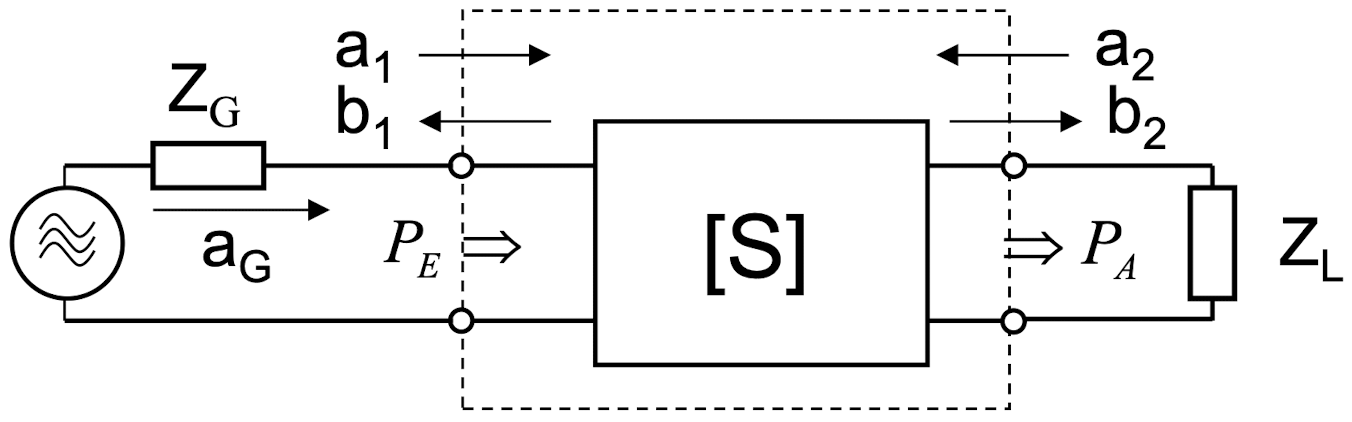
\includegraphics[width = 6cm]{./img/zweitorverstaerkung.png}\end{center}
	Eingangsleistung: $P_{E}=\left|a_{1}\right|^{2}-\left|b_{1}\right|^{2} =\left|a_{1}\right|^{2} \cdot\left(1-\left|\rho_{E}\right|^{2}\right)$\\
	Ausgangsleistung: $P_{A}=\left|b_{2}\right|^{2}-\left|a_{2}\right|^{2}=\left|b_{2}\right|^{2} \cdot\left(1-\left|\rho_{L}\right|^{2}\right)$\\

	Zusammenhang mit Generatorurwelle: $a_{1}=\frac{a_{G}}{1-\rho_{G} \rho_{E}}$\\

	Leistungsabgabe im Generator: $P_G = P_E = \left|a_{G}\right|^{2} \cdot \frac{1-\left|\rho_{E}\right|^{2}}{\left|1-\rho_{G} \rho_{E}\right|^{2}}$

	Maximale/verfügbare Generatorleistung für Anpassung ($\rho_{E}=\rho_{G}^{*}$):\\
	$P_{G V}=\frac{\left|a_{G}\right|^{2}}{1-\left|\rho_{G}\right|^{2}}$\\

	Übertragungsverhalten: $\frac{b_{2}}{a_{1}}=\frac{S_{21}}{1-\rho_{L} S_{22}}$\\

	Tatsächliche Leistungsverstärkung:\\
	$V_{P}=\frac{P_{A}}{P_{E}}=\frac{\left|b_{2}\right|^{2} \cdot\left(1-\left|\rho_{L}\right|^{2}\right)}{\left|a_{1}\right|^{2} \cdot\left(1-\left|\rho_{E}\right|^{2}\right)}=\frac{\left|S_{21}\right|^{2}}{\left|1-\rho_{L} S_{22}\right|^{2}} \cdot \frac{1-\left|\rho_{L}\right|^{2}}{1-\left|\rho_{E}\right|^{2}}$\\

	Übertragungsleistungsverstärkung/Gewinn\\(Ausgangsleistung bezogen auf verfügbare Generatorleistung):\\
	$G=\frac{P_{A}}{P_{G V}} = \frac{1-\left|\rho_{G}\right|^{2}}{\left|1-\rho_{G} \rho_{E}\right|^{2}} \cdot\left|S_{21}\right|^{2} \cdot \frac{1-\left|\rho_{L}\right|^{2}}{\left|1-\rho_{L} S_{22}\right|^{2}}$\\
	
	Wenn $Z_G = Z_L = Z_0$ $\rightarrow$ Anpassung: $\rho_G = \rho_L = 0$\\
	$\rightarrow$ $G = |S_{21}|^2$\\
	
	Maximale Leistungsverstärkung (maximaler Gewinn) bei Wirkleistungsanpassung am Eingang und Ausgang:
	$\rho_{G}=\rho_{E}^{*} ; \rho_{L}=\rho_{A}^{*}$\\

	Rückwirkungsfreiheit ($|S_{12}| / |S_{21}| < 0.1$): $\rho_{E} = S_{11}$\\

	\begin{emphbox}
		Gewinn rückwirkungsfreier Verstärker ($|S_{12}| / |S_{21}| < 0.1$), $\rho_{E}=S_{11}$:\\
		$G=\underbrace{\frac{1-\left|\rho_{G}\right|^{2}} {\left|1-\rho_{G} S_{11}\right|^{2}}}_{\text{Gewinn der Quelle}}\cdot \underbrace{\left|S_{21}\right|^{2}}_{\text {des Zweitors }} \cdot  \underbrace{\frac{1-\left|\rho_{L}\right|^{2}}{\left|1-\rho_{L} S_{22}\right|^{2}}}_{\text {der Last }}$\\
		
		Maximaler Gewinn für beidseitige Wirkleistungsanpassung: $\rho_{G}=\rho_{E}^{*}=S_{11}^{*} ; \rho_{L}=\rho_{A}^{*}=\rho_{G}^{*}=S_{22}^{*}$\\
		$G_{\max }=\frac{\left|S_{21}\right|^{2}}{\left(1-\left|S_{11}\right|^{2}\right) \cdot\left(1-\left|S_{22}\right|^{2}\right)}$
	\end{emphbox}
\end{sectionbox}	
\begin{sectionbox}
	\subsection{Anpassnetzwerke}
	\begin{itemize}
		\item Für maximalen Gewinn ist Wirkleistungsanpassung erforderlich
		\item HF-Verstärker haben frequenzabhängige und stark reaktive Ein/Ausgangsimpedanzen, die angepasst werden müssen
		\item Problem: Reaktive Anpassungen in der Regel schmalbandig
		\item Problem: Reflexionen können zu Stabilitätsproblemen führen
	\end{itemize}
\end{sectionbox}
\begin{sectionbox}
	\subsection{Absolute Stabilität}
	\begin{itemize}
		\item Die Tore verhalten sich unabhängig der passiven Beschaltung passiv
		\item Der Verstärker ist unabhängig von der Beschaltung stabil
	\end{itemize}
	Mathematisch: $\left|\rho_{E}\right|\le1$ für $\left|\rho_{L}\right|\le1 \quad \wedge \quad\left|\rho_{A}\right|\le1$ für $\left|\rho_{G}\right|\le1$\\
	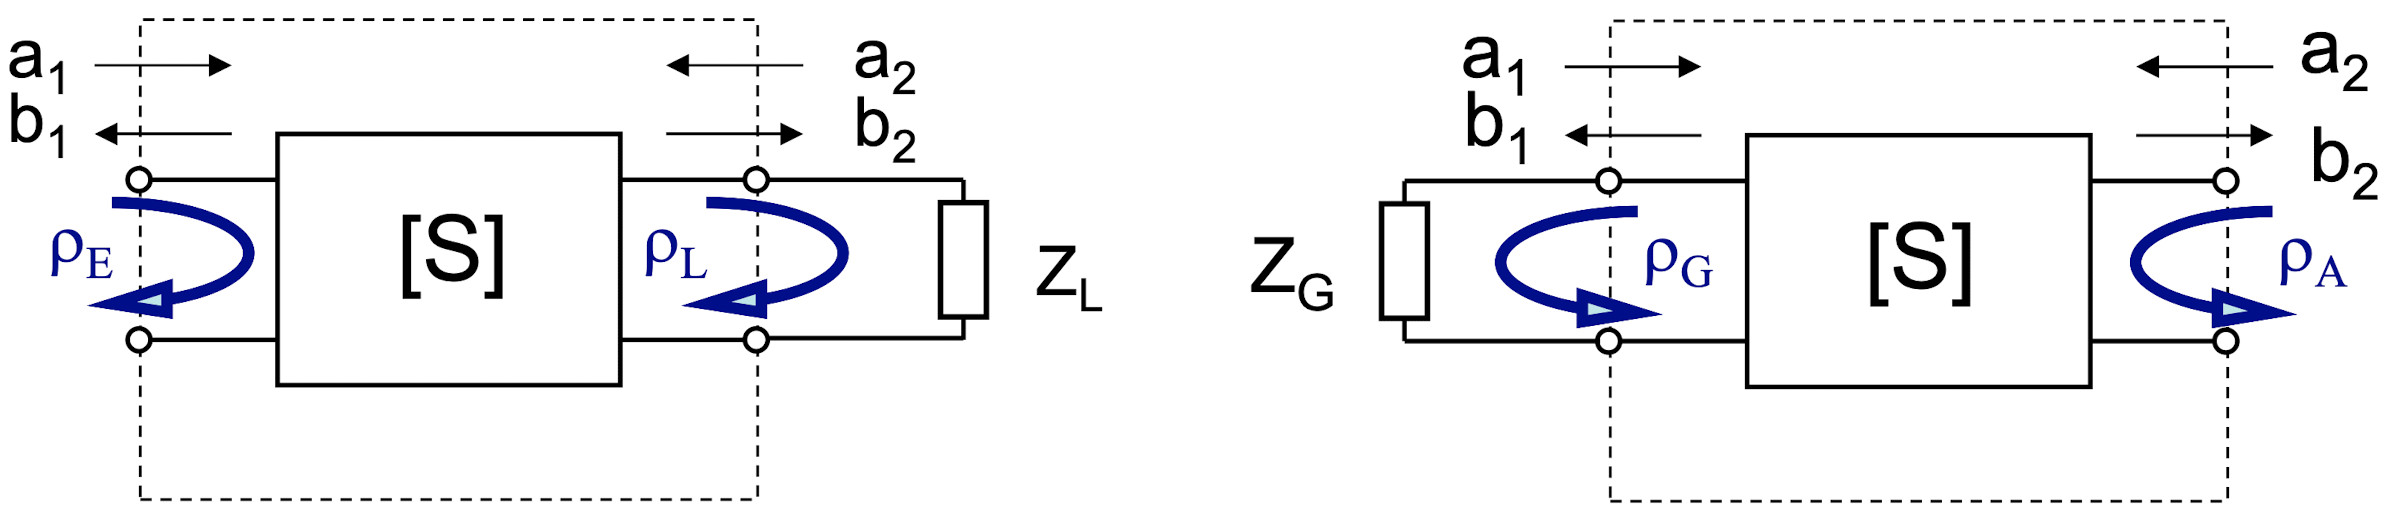
\includegraphics[width = 6.8cm]{./img/stablilitaet.png}\\
	\begin{emphbox}
		5 notwendige und hinreichende Bedingungnen für absolute Stabilität:\\
		\begin{enumerate}
			\item $\left|S_{11}\right|<1$ und $\left|S_{22}\right|<1$
			\item $\left|S_{12} \cdot S_{21}\right|<1-\left|S_{22}\right|^{2}$ und $\left|S_{12} \cdot S_{21}\right|<1-\left|S_{11}\right|^{2}$
			\item $K > 1$
		\end{enumerate}
		Stabilitätsfaktor:\\
		$K=\frac{1+\left|S_{11} \cdot S_{22}-S_{12} \cdot S_{21}\right|^{2}-\left|S_{11}\right|^{2}-\left|S_{22}\right|^{2}}{\left|2 \cdot S_{12} \cdot S_{21}\right|}$
	\end{emphbox}

	\textbf{Stabilitätskreise}:\\
	Zur Überprüfung wird die Ortskurve $\left|\rho_{L}\right|=1$ bzw $\left|\rho_{G}\right|=1$ zum Ein- /Ausgang transformiert:\\
	$\left|\rho_{E}\right|=\left|s_{11}+\frac{s_{12} \cdot s_{21} \rho_{L}}{1-s_{22} \rho_{L}}\right| \stackrel{!}{=} 1$ ($\rho_L$-Ebene) eingangseitige Stab.\\
	$\left|\rho_{A}\right|=\left|s_{22}+\frac{s_{12} \cdot s_{21} \rho_{G}}{1-s_{11} \rho_{G}}\right| \stackrel{!}{=} 1$ ($\rho_G$-Ebene) ausgangseitige Stab.
	$C_L, R_L$: alle $\rho_L$ auf Kreis $(C_L, R_L)$ ergeben einen Eingangsreflexionsfaktor $|\rho_E| = 1$\\
	$C_G, R_G$: alle $\rho_G$ auf Kreis $(C_G, R_G)$ ergeben einen Eingangsreflexionsfaktor $|\rho_A| = 1$
	\begin{emphbox}
		Bild des Eingangsreflexionsfaktors in der Lastebene:\\
		$C_{L}=\frac{\left(S_{22}-\Delta_{S} S_{11}^{*}\right)^{*}}{\left|S_{22}\right|^{2}-\left|\Delta_{S}\right|^{2}}$, 
		$R_{L}=\left|\frac{S_{12} S_{21}}{\left|S_{22}\right|^{2}-\left|\Delta_{S}\right|^{2}}\right|$\\
		Bild des Ausgangsreflexionsfaktors in der Eingangsebene:\\
		$C_{G}=\frac{\left(S_{11}-\Delta_{S} S_{22}^{*}\right)^{*}}{\left|S_{11}\right|^{2}-\left|\Delta_{S}\right|^{2}}$, $R_{G}=\left|\frac{S_{12} S_{21}}{\left|S_{11}\right|^{2}-\left|\Delta_{S}\right|^{2}}\right|$\\
		\vspace{1em}
		With $\Delta_{S} = det(S) = S_{11}S_{22}-S_{12}S_{21}$
	\end{emphbox}
	\comment{Kriterium für die Wahl der stabilen Seite hinzufügen.}\\
	\comment{Einfügen von Widerständen zur Stabilisierung hinzufügen.}\\ 
	Finden eines Punktes der stabil sein muss. Das ist bei Anpassung. z.B. $\rho_L=S^*_{22}$
\end{sectionbox}

\begin{sectionbox}
	\subsection{Leitungskoppler}
	\begin{itemize}
		\item Innenleiter zweier Leitungssysteme werden über Strecke $l$ aufeinander angenähert und parallel geführt
		\item Verwendung von TEM Leitungen $\rightarrow$ Phasengeschwindigkeiten der verschiedenen Eigenwellen sind gleich !wesentliche Eigenschaft
		\item Homogenes Dielektrikum zwischen den Platten
		\item Doppelte Symmetrie ermöglicht Gleich/Gegentaktanalyse
		\item Alle Koppler mit doppelter Symmetrie und $z_ez_d = 1$ sind allseits angepasst und $S_{31} = S_{13} = 0$
		\item Alle verlustfreien angepassten Koppler mit doppelter Symmetrie sind $90^{\circ}$ Koppler
		\item Können zur Signaldämpfung eingesetzt werden
	\end{itemize}
	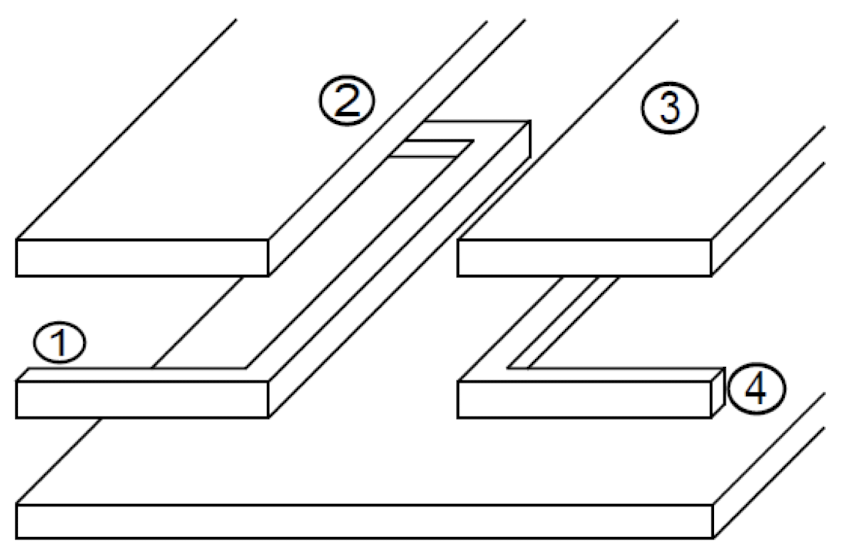
\includegraphics[width = 2.5cm]{./img/leitungskoppler1.png}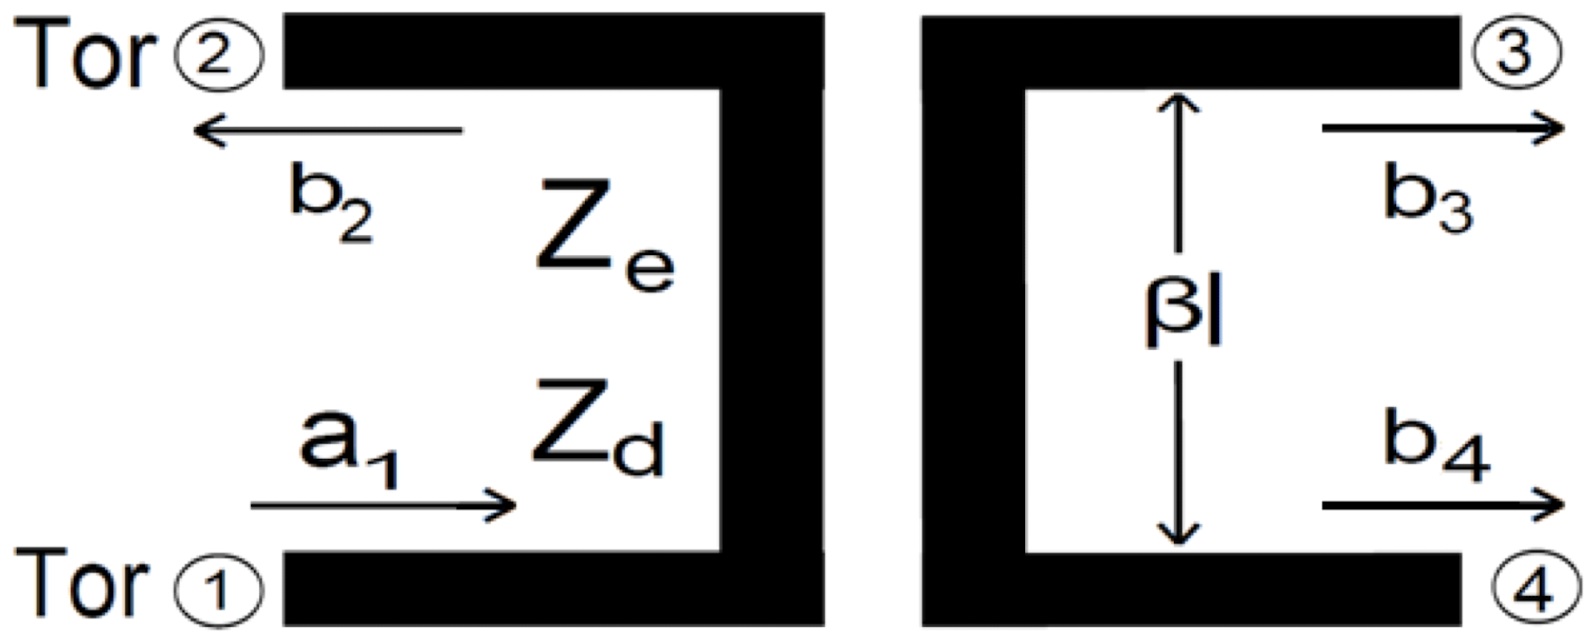
\includegraphics[width = 4.3cm]{./img/leitungskoppler2.png}\\
	 
	\textbf{Gleich/Gegentaktanalyse}:\\
	Für $a_2 = a_3 = 0$ werden Wellen in Tor 1 und 4 eingespeist. Aufgrund der Symmetrie muss nur ein Ast des Kopplers betrachtet werden.\\
	Gleichtakt: $a_1^+ = a_4^+ = \frac{a_1}{2}$ $\rightarrow$ Tor 1 sieht Leitung mit Impedanz $Z_e$.\\
	Gegentakt: $a_1^- = -a_4^- = \frac{a_1}{2}$ $\rightarrow$ Tor 1 sieht Leitung mit $Z_d$.\\
	Bei Überlagerung gilt $a_4 = 0$ und dank doppelter Symmetrie $S_{ii} = S_{jj}$, $S_{12} = S_{21} = S_{34} = S_{43}$ usw. kann $[S]$ bestimmt werden.

	\begin{emphbox}
		Koppelgrößen für $z_e z_d = 1$:\\
		\vspace{1em}
		$S_{21}=\frac{2}{2 \cos \beta l+j\left(z_{e}+\frac{1}{z_{e}}\right) \sin \beta l}$\\
		$S_{41}=\frac{j\left(z_{e}-\frac{1}{z_{e}}\right) \sin \beta l}{2 \cos \beta l+j\left(z_{e}+\frac{1}{z_{e}}\right) \sin \beta l}$
		\begin{itemize}
			\item $S_{11} = S_{31} = 0$ \textbf{frequenzunabhängig}
			\item $S_{21}$ und $S_{41}$ unterscheiden sich \textbf{frequenzunabhängig} um $90^\circ$
		\end{itemize}
	\end{emphbox}
\end{sectionbox}
\begin{sectionbox}
	\subsection{Bandbreite von 3dB-Leitungskopplern}
	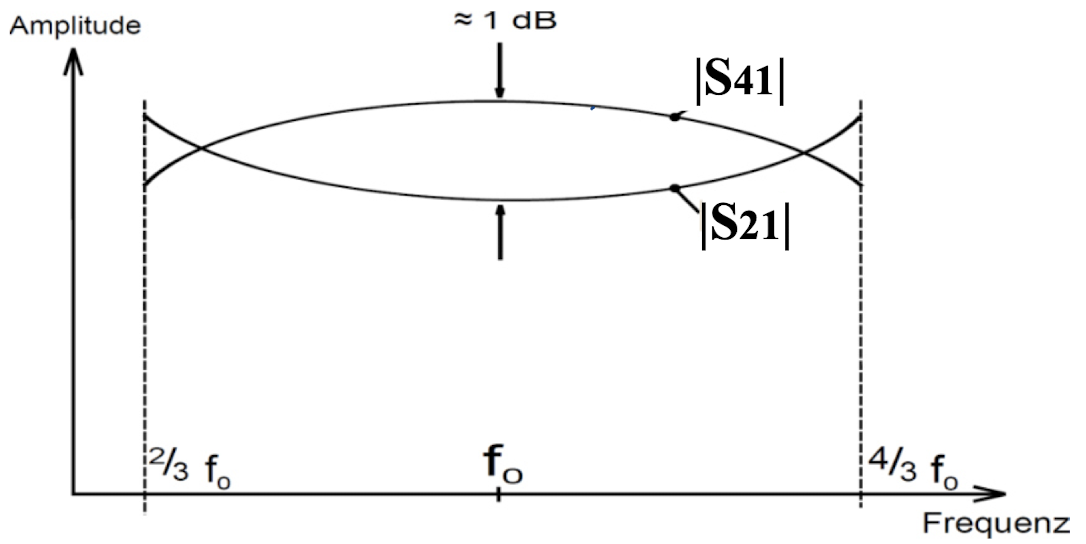
\includegraphics[width = 4.3cm]{./img/leitungskoppler_bb.png}\raisebox{5mm}{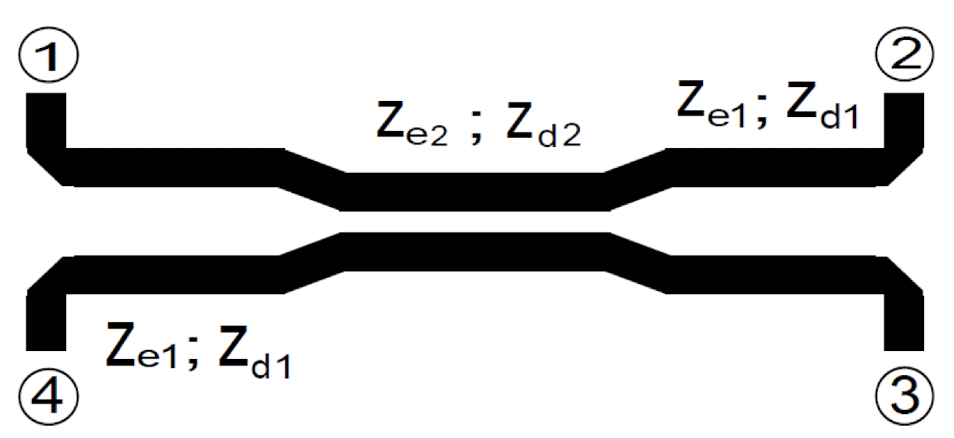
\includegraphics[width = 2.4cm]{./img/leitungskoppler_ms.png}}\\
	Etwa eine halbe Oktave Bandbreite, bei max. 1dB Unterschied.\\
	Mehrstufige Koppler verbessern die Bandbreite.
\end{sectionbox}
\begin{sectionbox}
	\subsection{Resistive Koppler}
	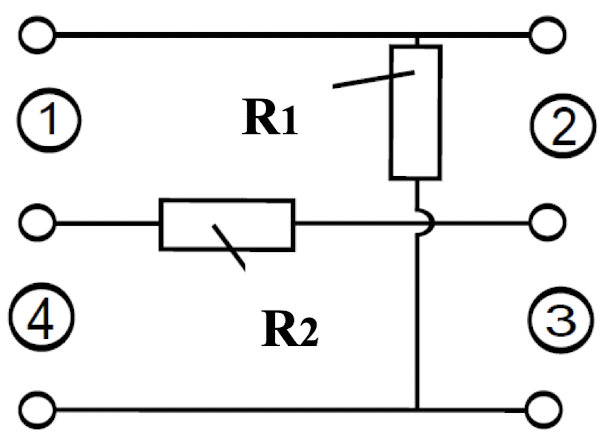
\includegraphics[width = 4.3cm]{./img/resistiver_koppler.png}
	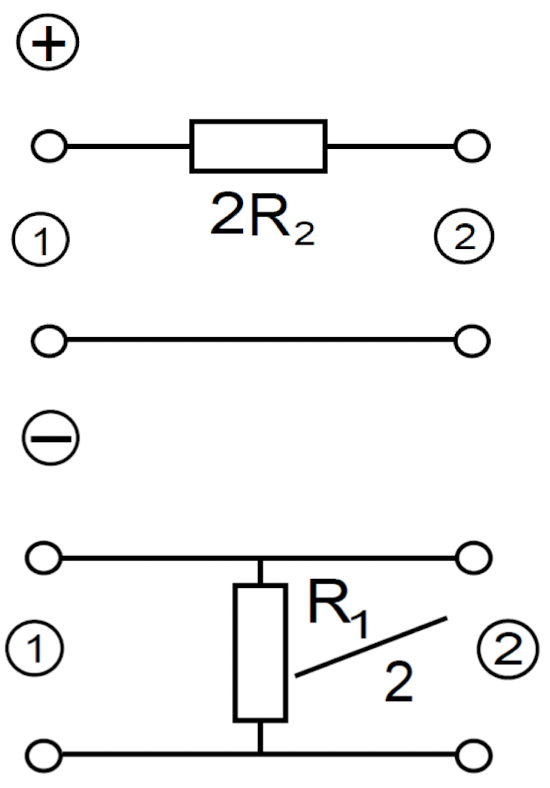
\includegraphics[width = 2.3cm]{./img/resistiver_koppler_evenodd.png}\\
	Schließt man alle Tore mit $Z_0$ ab, ergibt sich eine Wheatstone-Brücke.\\
	\begin{emphbox}
		Mit $R_1 R_2 = Z_0^2$:\\
		\vspace{1em}
		Anpassung: $S_{11}=S_{22}=S_{33}=S_{44}=0$\\
		Isolation: $S_{31}=S_{13} = S_{42} = S_{24} =0$\\
		Übertragung: $S_{21}=\frac{Z_{0}}{Z_{0}+R_{2}} \quad S_{41}=\frac{R_{2}}{Z_{0}+R_{2}}$
	\end{emphbox}
	\begin{itemize}
		\item Phasen von $S_{21}$ und $S_{41}$ gleich: $0^{\circ}$-Koppler
		\item Für $R_{1}=R_{2}=Z_{0}$ 6dB Dämpfung nach Tor 2, bzw. Tor 4.
		\item Für $R_1 = j \omega L$, $R_2 = 1 / j \omega C$, $R_1R_2 = Z_0^2$ ist der Koppler verlustlos, breitbandig zu Tor 3 entkoppelt, aber die Übertragung ist frequenzabhängig.
		\item Problem der Wheatstone-Brücke: nur ein Punkt geerdet $\rightarrow$ Symmetrieglied erforderlich $\rightarrow$ Bandbreite begrenzt
	\end{itemize}
\end{sectionbox}
\begin{sectionbox}
	\subsection{Null-Grad-Koppler (Wilkinsonteiler)}
	\begin{center}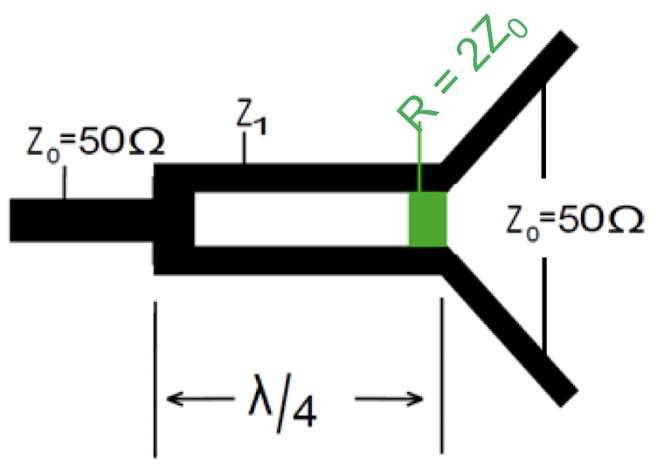
\includegraphics[width = 4cm]{./img/wilkinsonteiler.png}\end{center}
	\begin{itemize}
		\item Zur Transformation von $Z_0$ auf $2Z_0$ muss gelten $Z_1 = \sqrt{2}Z_0$
		\item Bei gekoppelten Leitungen ist $Z_1$ die Leitungsimpedanz der Gleichtaktwelle
		\item Bei Speisung an Tor 1 sind Tor 2 und 3 gleich in Amplitude und Phase
		\item wird $0^{\circ}$ Koppler genannt
		\item $R$ idealerweise verlustfrei da zwischen Punkten gleichen Potential
		\item Für $R = 2Z_0$ sind die Tore 2 und 3 entkoppelt
		\item Etwa eine Oktave Bandbreite, erweiterbar durch mehrere Stufen
	\end{itemize}
\end{sectionbox}

\section{Einige Theoreme der Elektromagnetischen Feldtheorie}
\begin{sectionbox}
	\subsection{Energiedichte im Feld}
	Herleitung aus der mechanischen Arbeit durch Anhhäherung von Ladung aus dem Unendlichen.\\
	Energiedichte des elektrischen Felds:\\
	$w_{e}=\int_{0}^{\vec{d}} \vec{e}^{\prime} \cdot d \vec{d}^{\prime}= \frac{1}{\varepsilon_{r} \varepsilon_{0}} \frac{1}{2}|\vec{d}|^{2}=\frac{1}{2} \varepsilon_{r} \varepsilon_{0}|\vec{e}|^{2}$\\
	Energiedichte des magnetischen Felds:\\
	$w_{m}=\frac{1}{\mu_{r} \mu_{0}} \int_{0}^{d} \vec{b}^{\prime} \cdot d \vec{b}^{\prime}=\frac{1}{\mu_{r} \mu_{0}} \frac{1}{2}|\vec{b}|^{2}= \frac{1}{2} \mu_{r} \mu_{0}|\vec{h}|^{2}$\\
	(Die letzten beiden Umformungen gelten für lineares isotropes Material.)
\end{sectionbox}

\begin{sectionbox}
	\subsection{Elektromagnetische Energiebilanz im Zeitbereich}
	\begin{emphbox}
	$\underbrace{-\frac{\partial}{\partial t}\left(W_{e}+W_{m}\right)}_{\substack{\text{zeitliche Änderung der}\\ \text{in} V \text{gespeicherten Energie}}}=\underbrace{p_{\kappa}}_{\text{Verlustleistung}}+\underbrace{p_{s}}_{
		\substack{\text{aus(+)- oder}\\\text{eingebrachte(-)}\\ \text{Leistung}}
	}$\\
	\end{emphbox}
	\textbf{Stationäres Feld}:
	$-\frac{\partial}{\partial t}\left(W_{e}+W_{m}\right)=0 \quad \rightarrow \quad p_{\kappa}=-p_{s}$

	\begin{tablebox}{@{\hspace{0mm}}l@{\extracolsep\fill}l@{\hspace{10mm}\extracolsep\fill}}
		d. $A$ austretende Leist.: & $p_{s}=\oiint\limits_{A(V)} [\vec{e} \times \vec{h}] \cdot d \vec{A} = \oiint\limits_{A(V)} \vec{s} \cdot d \vec{A}$ \\
		ohmsche Verlustleistung: & $p_{\kappa}=\iiint\limits_{V}[\kappa \vec{e} \cdot \vec{e}] d v$\\
		elektrische Energie in V: & $W_{e}=\iiint\limits_{V}\left[\frac{1}{2} \varepsilon_{r} \varepsilon_{0}|\vec{e}|^{2}\right] d v \quad=\iiint\limits_{V} w_{e} d v$\\
		magnetische Energie in V: & $W_{m}=\iiint\limits_{V}\left[\frac{1}{2} \mu_{r} \mu_{0}|\vec{h}|^{2}\right] d v=\iiint\limits_{V} w_{m} d v$\\
	\end{tablebox}	
	Mit Pointing Vektor (Leistungsflussvektor): $\vec{s} = \vec{e} \times \vec{h}$ $\left[\frac{W}{m^2}\right]$\\
	(Herl. über Erweiterung der MWG mit $\vec{e}$, $\vec{h}$, Satz v. Gauss und Subtr.)
\end{sectionbox}
\begin{sectionbox}
	\subsection{Elektromagnetische Energiebilanz in Zeigerdarstellung}
	\begin{emphbox}
	$-\oiint\limits_{A(V)} \vec{S} \cdot d \vec{A}=P_{V}-2 j \omega\left(\bar{W}_{e}-\bar{W}_{m}\right)$\\
	\end{emphbox}
	Wirkleistungsfluss durch A (Verlustleistung in V): $P_{V}=P_{\kappa}+P_{\varepsilon}+P_{\mu}$

	\begin{tablebox}{@{\hspace{0mm}}l@{\extracolsep\fill}l@{\hspace{10mm}\extracolsep\fill}}
		ohmsche Verlustleistung: & $P_{\kappa}=\frac{1}{2} \iiint\limits_{V}\left[\kappa \vec{E} \cdot \vec{E}^{*}\right] d v$\\
		dielektrische Verlustleistung: & $P_{\varepsilon}=\frac{1}{2} \iiint\limits_{V}\left[\omega \varepsilon_{r}^{\prime \prime} \varepsilon_{0} \vec{E} \cdot \vec{E}^{*}\right] d v$\\
		magnetische Verlustleistung: & $P_{\mu}=\frac{1}{2} \iiint\limits_{V}\left[\omega \mu_{r}^{\prime \prime} \mu_{0} \vec{H} \cdot \vec{H}^{*}\right] d v$\\
		mittlere elektrische Energie: & $\bar{W}_{e}=\frac{1}{4} \iiint\limits_{V}\left[\varepsilon_{r}^{\prime} \varepsilon_{0} \vec{E} \cdot \vec{E}^{*}\right] d v$\\
		mittlere magnetische Energie: & $\bar{W}_{m}=\frac{1}{4} \iiint\limits_{V}\left[\mu_{r}^{\prime} \mu_{0} \vec{H} \cdot \vec{H}^{*}\right] d v$\\
	\end{tablebox}	
	Komplexer Pointing Vektor: $\vec{S}=\frac{1}{2} \vec{E} \times \vec{H}^{*}$\\
	$\frac{1}{2} \operatorname{Re}\left(\vec{E} \times \vec{H}^{*}\right)=\overline{\vec{e}(t) \times \vec{h}(t)}=\frac{1}{T} \int_{0}^{T}(\vec{e}(t) \times \vec{h}(t)) d t$\\
\end{sectionbox}
\begin{sectionbox}
	\subsection{Eindeutigkeitstheorem}
	\textbf{Frage}: Unter welchen Voraussetzungen (Randbedingungnen) ist die Feldlösung in einem durch $A$ geschlossenen Lösungsgebiet für eine Anregung eindeutig bestimmt?\\
	\begin{center}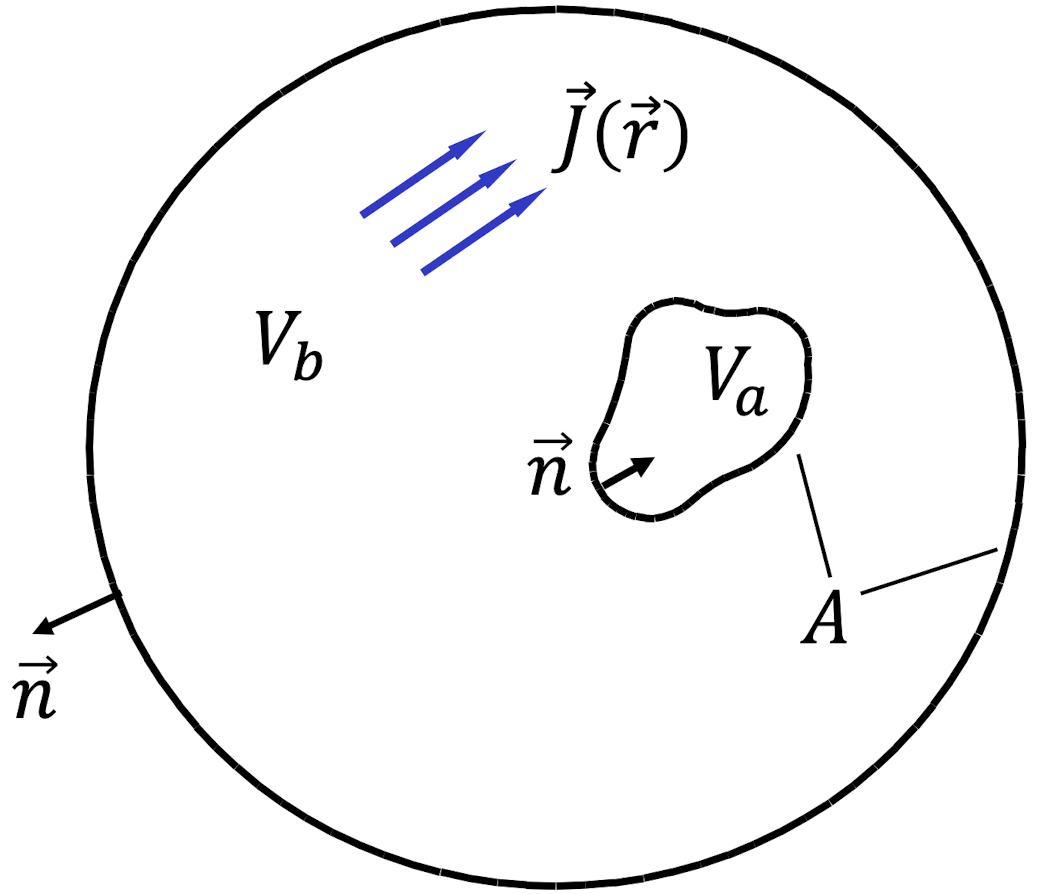
\includegraphics[width = 4cm]{./img/eindeutigkeitsthm.png}\end{center}
	\textbf{Ansatz}: Nehme an, es gäbe zwei Feldlösungen der MWG $\vec{E}_1, \vec{H}_1$ und $\vec{E}_2, \vec{H}_2$ im gleichen Gebiet $V_b$ mit gleicher Anregung $\vec{J}, \vec{M}$. Durch Differenzbildung der Lösungen, Einsetzen in die MWG (1-2), und Erweiterung mit $\delta \vec{H}^{*}$ bzw. $\delta \vec{E}$, Differenzbildung, Satz v. Gauß ergibt sich:
 	$\iiint_{V_{b}} \nabla \cdot\left(\delta \vec{E}(\vec{r}) \times \delta \vec{H}^{*}(\vec{r})\right) d v \quad=\oiint_{A}\left(\delta \vec{E}(\vec{r}) \times \delta \vec{H}^{*}(\vec{r})\right) \cdot d\vec{a} = \iiint_{V_{b}}\left[-j \omega \mu(\vec{r})|\delta \vec{H}(\vec{r})|^{2}+j \omega \varepsilon^{*}(\vec{r})|\delta \vec{E}(\vec{r})|^{2}\right] d v$.\\
	Oberflächenintegral verschwindet für:
	%\vspace{-1em}
	\begin{tablebox}{@{\hspace{2mm}}l@{\extracolsep\fill}}
		1. Vorgabe von $\vec{n} \times \vec{E}$ auf $A$ \\
		2. Vorgabe von $\vec{n} \times \vec{H}$ auf $A$ \\
		3. Vorgabe von $\vec{n} \times \vec{E}$ auf Teilen v. $A$ und $\vec{n} \times \vec{H}$ auf dem Rest
	\end{tablebox}
	Bei verschwindendem Oberflächenintegral:\\
	$\Rightarrow$ Für $\mu^{\prime \prime}(\vec{r})>0 $ und/oder $ \varepsilon^{\prime \prime}(\vec{r})>0$ ist die Feldlösung eindeutig.\\
	$\Rightarrow$ Für verlustfreie Medien (ideale Resonatoren) oder negativen Materialien existieren mehrere Lösungen.

\end{sectionbox}	

\begin{sectionbox}
	\subsection{Reziprozität}
	Betrachte Quellen $\vec{J}_{1}, \vec{M}_{1}$ mit dem Feld $\vec{E}_{1}, \vec{H}_{1}$ und\\
	Betrachte Quellen $\vec{J}_{2}, \vec{M}_{2}$ mit dem Feld $\vec{E}_{2}, \vec{H}_{2}$ mit MWG:\\
	\begin{tablebox}{@{\hspace{0mm}}l@{\extracolsep\fill}l@{\hspace{10mm}\extracolsep\fill}}
		(1) $\nabla \times \vec{H}_{1}=j \omega \varepsilon \vec{E}_{1}+\vec{J}_{1}$ & (3) $\nabla \times \vec{H}_{2}=j \omega \varepsilon \vec{E}_{2}+\vec{J}_{2}$ \\
		(2) $\nabla \times \vec{E}_{1}=-j \omega \mu \vec{H}_{1}-\vec{M}_{1}$ & (4) $\nabla \times \vec{E}_{2}=-j \omega \mu \vec{H}_{2}-\vec{M}_{2}$
	\end{tablebox}
	\textbf{Annahmen:}: Materialien sind isotrop (trotzdem gg. ortsabhängig).\\
	\textbf{Ansatz}: Berechne $(3) \cdot \vec{E}_{1}-(2) \cdot \vec{H}_{2} - ((1) \cdot \vec{E}_{2}-(4) \cdot \vec{H}_{1})$. RHS liefert Beiträge nur in Quellregionen. Satz v. Gauss. Ergebnis:\\
	\begin{emphbox}
		$-\oiint\limits_{A(V)}\left(\vec{E}_{1} \times \vec{H}_{2}-\vec{E}_{2} \times \vec{H}_{1}\right) \cdot d \vec{A}=\iiint\limits_{V}\left(\vec{E}_{1} \cdot \vec{J}_{2}+\vec{H}_{2} \cdot \vec{M}_{1}-\vec{E}_{2} \cdot \vec{J}_{1}-\vec{H}_{1} \cdot \vec{M}_{2}\right) d v$
	\end{emphbox}
	\begin{emphbox}
		\textbf{Für Quellefreie Gebiete}:\\
		Diff. Form: $-\nabla \cdot\left(\vec{E}_{1} \times \vec{H}_{2}-\vec{E}_{2} \times \vec{H}_{1}\right)=0$\\
		Integralform: $\oiint\limits_{A(V)}\left(\vec{E}_{1} \times \vec{H}_{2}-\vec{E}_{2} \times \vec{H}_{1}\right) \cdot d \vec{A}=0$
	\end{emphbox}
	Wähle $A(V)$ als die Fernkugeloberfläche $r \rightarrow \infty$ (lokale ebene Welle).\\
	$E_{\vartheta}=Z H_{\varphi}$ u. $E_{\varphi}=-Z H_{\vartheta}$, das Oberflächenintegral verschwindet:\\
	\begin{emphbox}
		$\iiint\limits_{V}\left(\vec{E}_{1} \cdot \vec{J}_{2}-\vec{H}_{1} \cdot \vec{M}_{2}\right) d v=\iiint\limits_{V}\left(\vec{E}_{2} \cdot \vec{J}_{1}-\vec{H}_{2} \cdot \vec{M}_{1}\right) d v$
	\end{emphbox}

	\textbf{Für idealen elektrischen Leiter (PEC)}:\\
	Da keine mag. Ströme existieren: $\vec{M}_{1} = \vec{M}_{2} = 0$.\\
	Betrachte eingeprägten Strom $\vec{J}_{1}$ im PEC $\rightarrow$ $\vec{E}_{1} = 0$ (PEC) $\rightarrow$ Integral ist $0$ $\rightarrow$ $\vec{E}_{2} = 0$ für beliebige $\vec{J}_{2} = 0$.\\
	
	$\Rightarrow$ Elektrischer Strom $\vec{J}$ auf/in PEC straht kein Feld ab.\\
	$\Rightarrow$ Magnetischer Strom $\vec{M}$ auf/in PMC straht kein Feld ab.\\
\end{sectionbox}

\begin{sectionbox}
	\subsection{Reziprozität von Antennen}
	Betrachte zwei beliebige metallische PEC Antennen (auch für nicht-PEC):\\
	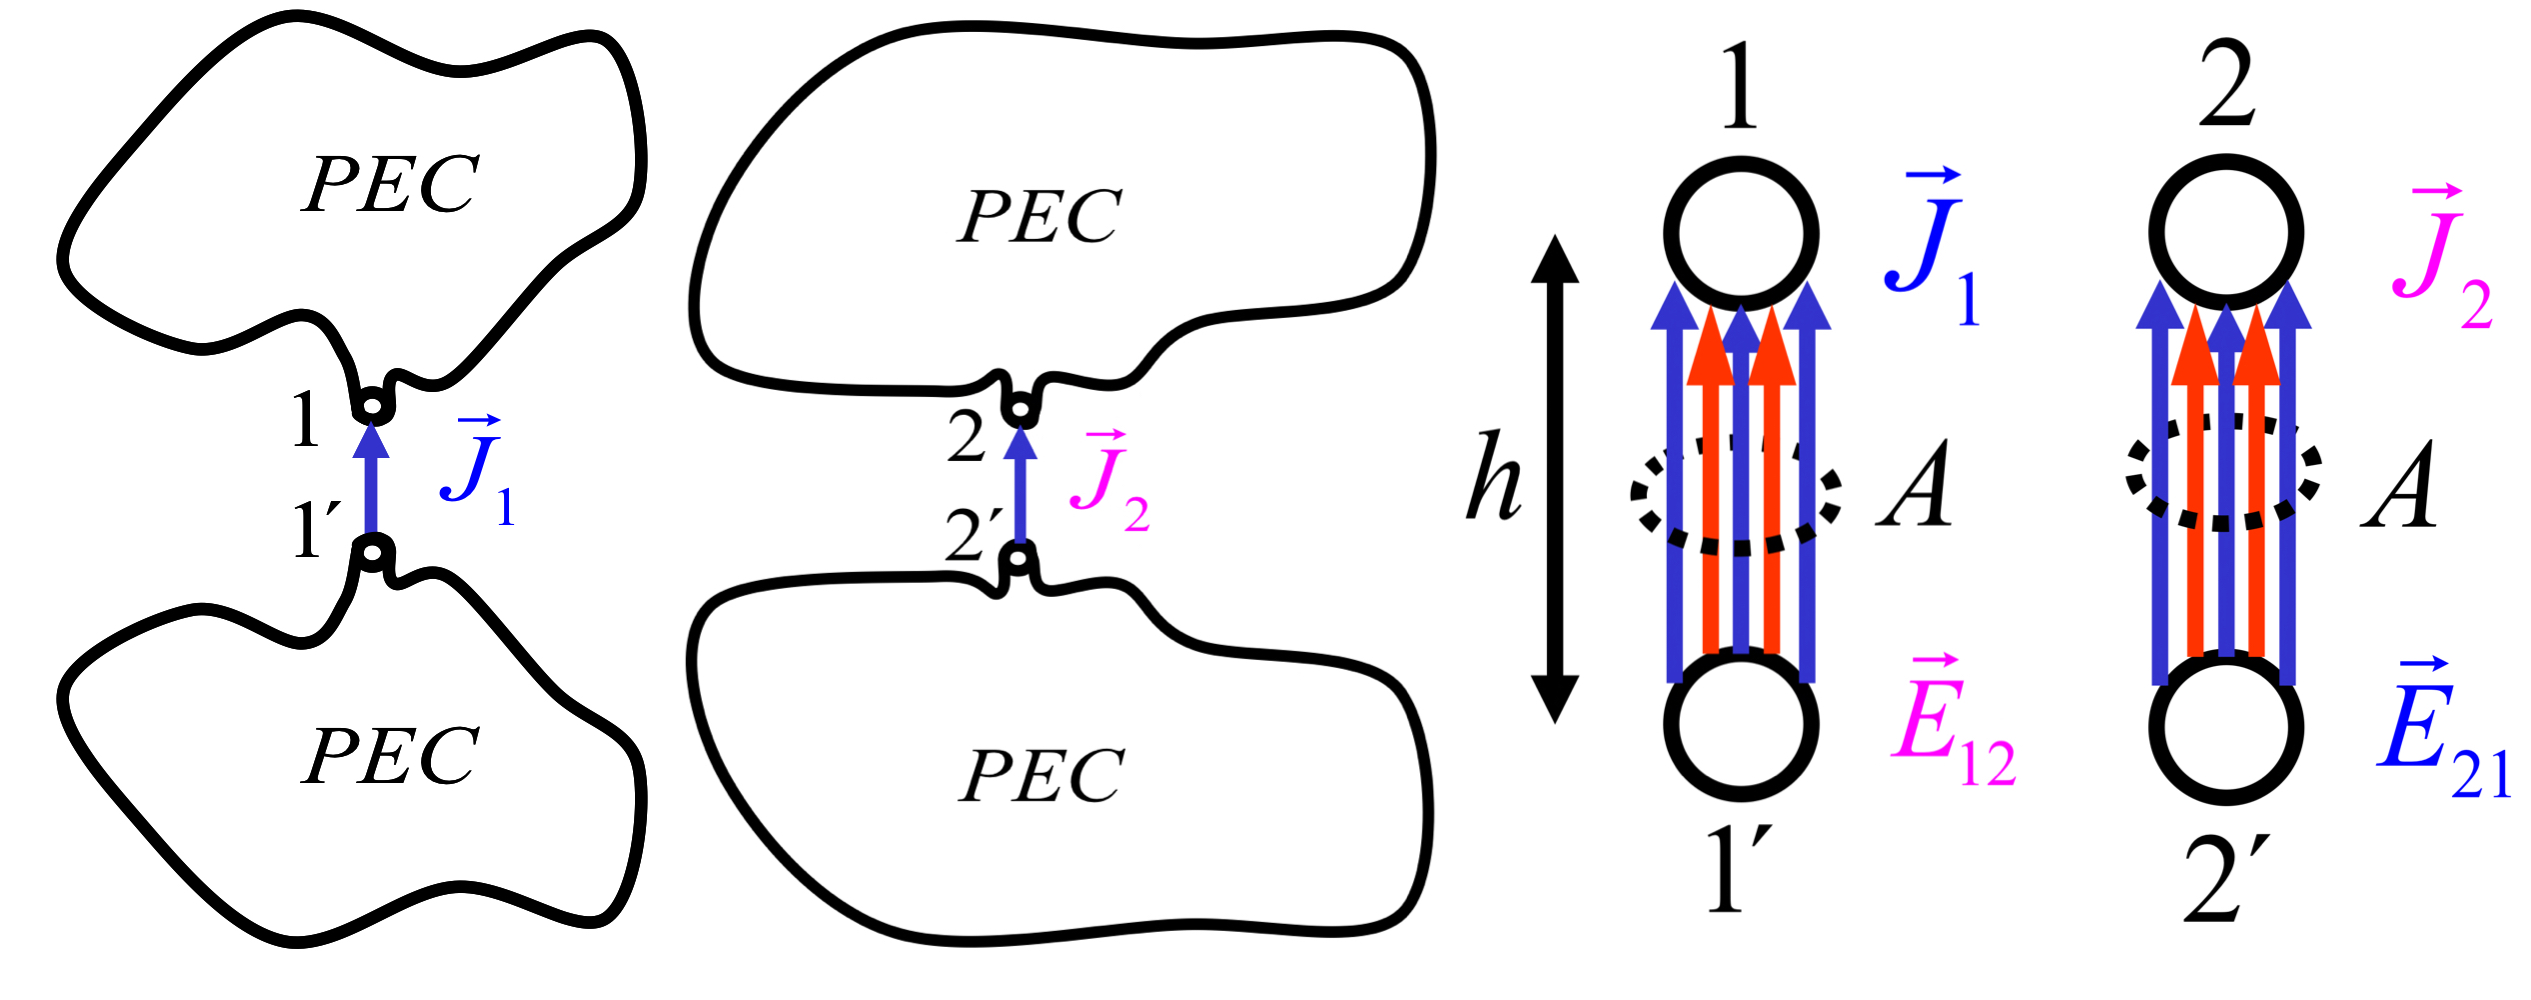
\includegraphics[width = 6.8cm]{./img/reziproke_antennen.jpeg}\\

	Nutze $\iiint\limits_{V}\left(\vec{E}_{12} \cdot \vec{J}_{1}\right) d v=\iiint\limits_{V}\left(\vec{E}_{21} \cdot \vec{J}_{2}\right) d v$.\\
	Weitere Annahmen: $\vec{J}_{1} \neq \vec{f}(h)$ u. $\vec{E}_{12}=\text { konst. } \text { in } A$\\$\Rightarrow$ $\int \vec{E}_{12} \cdot d \vec{h}=-U_{10} \quad \iint \vec{J}_{1} \cdot d \vec{A}=I_{1}$\\
	\begin{emphbox}
		$\frac{U_{10}}{I_{2}}=Z_{12}=\frac{U_{20}}{I_{1}}=Z_{21}$
	\end{emphbox}
\end{sectionbox}

\begin{sectionbox}
	\subsection{Elektromagnetische Potentiale}
	Zerlegung in elektrische und magnetische Felder:
	\begin{center}$\vec{E} = \vec{E}_{e} + \vec{E}_{m} \qquad \vec{H} = \vec{H}_{e} + \vec{H}_{m}$\end{center}
	\begin{tablebox}{@{\hspace{0mm}}l@{\extracolsep\fill}l@{\hspace{0mm}\extracolsep\fill}}
		\textbf{Elektrische Ströme} & \textbf{Magnetische Ströme}\\
		\hline
		MWG: & \\
		$\begin{aligned}
			\nabla \times \vec{H}_{e} &=j \omega \varepsilon \vec{E}_{e}+\vec{J} \\
			\nabla \times \vec{E}_{e} &=-j \omega \mu \vec{H}_{e} \\
			\nabla \cdot\left(\varepsilon \vec{E}_{e}\right) &=\rho \\
			\nabla \cdot\left(\mu \vec{H}_{e}\right) &=0
			\end{aligned}$ & $\begin{aligned}
				-\nabla \times \vec{E}_{m} &=j \omega \mu \vec{H}_{m}+\vec{M} \\
				\nabla \times \vec{H}_{m} &=j \omega \varepsilon \vec{E}_{m} \\
				\nabla \cdot\left(\mu \vec{H}_{m}\right) &=\rho_{m} \\
				\nabla \cdot\left(\varepsilon \vec{E}_{m}\right) &=0
				\end{aligned}$\\
		\hline
		Felddarstellung über Potentiale: & \\
		$\begin{aligned}
			\vec{H}_{e}(\vec{r}) &=\frac{1}{\mu} \nabla \times \vec{A}(\vec{r}) \\
			\vec{E}_{e}(\vec{r}) &=-j \omega \vec{A}-\nabla \phi
			\end{aligned}$ & $\begin{aligned}
				\vec{E}_{m}(\vec{r}) &=-\frac{1}{\varepsilon} \nabla \times \vec{F}(\vec{r}) \\
				\vec{H}_{m}(\vec{r}) &=-j \omega \vec{F}-\nabla \psi 
				\end{aligned}$\\
			$=-j \omega\left(\vec{A}(\vec{r})+\frac{1}{k^{2}} \nabla \nabla \cdot \vec{A}(\vec{r})\right)$ & $=-j \omega\left(\vec{F}(\vec{r})+\frac{1}{k^{2}} \nabla \nabla \cdot \vec{F}(\vec{r})\right)$\\
		\hline
		Lorenz-Eichung: & \\
		$\nabla \cdot \vec{A}(\vec{r})+j \omega \mu \varepsilon \phi(\vec{r})=0$ & $\nabla \cdot \vec{F}(\vec{r})+j \omega \mu \varepsilon \psi(\vec{r})=0$\\
		\hline
		Helmholtz-Gleichungen: & \\
		$\begin{aligned}
			&\Delta \vec{A}(\vec{r})+k^{2} \vec{A}(\vec{r})=-\mu \vec{J}(\vec{r}) \\
			&\Delta \phi(\vec{r})+k^{2} \phi(\vec{r})=-\frac{\rho(\vec{r})}{\varepsilon}
			\end{aligned}$ & $\begin{aligned}
				&\Delta \vec{F}(\vec{r})+k^{2} \vec{F}(\vec{r})=-\varepsilon \vec{M}(\vec{r}) \\
				&\Delta \psi(\vec{r})+k^{2} \psi(\vec{r})=-\frac{\rho_{m}(\vec{r})}{\mu}
				\end{aligned}$\\
	\end{tablebox}
	\textbf{Idee:} \comment{Kurze Beschreibung der Vorteile der Darstellung (Entkopplung v. Gleichungen, Entfernen von Redundanz in MWG, Modellierungsfreiheit, Green'sche Funktionen skalar)}
\end{sectionbox}
\begin{sectionbox}
	\subsection{Dualität}
	Besitzen zwei Gleichungssysteme, die unterschiedliche physikalische Phänomene beschreiben, die gleiche mathematische Form, so nehmen ihre Lösungen die gleiche mathematische Form an.

	Felder elektrischer Quellen sind dual zu Feldern magnetischer Quellen.\\
	Duale Lösungen erfordern zueinander duale Randbedingungen.\\
	\textbf{Anwendungen:}
	\begin{itemize}
		\item Verifizierung von zueinander dualen Gleichung und Lösungen.
		\item Ersetzen von Größen in einer Lösung durch duale Größen führt zur dualen Lösung.
	\end{itemize}
\end{sectionbox}

\begin{sectionbox}
	\subsection{Green'sche Funktionen}

\end{sectionbox}

\begin{sectionbox}
	\subsection{Huygens'sches Prinzip}
	\textbf{Idee}: Das Feld einer Primärquelle im Gebiet $V_a$ kann durch äquivalente Oberflächenströme $\vec{J}_A$, $\vec{M}_A$ auf der Grenzfläche $A(V_b)$ ersetzt werden. $V_a$ wird dadurch feldfrei und kann mit beliebigen Materialien (zb. PEC) gefüllt werden. Die Flächenströme sind Sekundärquellen, die zur Berechnung des Felds in $V_b$ verwendet werden können.\\
	$\begin{aligned}
		&\vec{E}(\vec{r})=\iiint\limits_{V_{b}}\left[\overleftrightarrow{G}_{J}^{E}\left(\vec{r}, \vec{r}^{\prime}\right) \cdot \vec{J}\left(\vec{r}^{\prime}\right)+\overleftrightarrow{G}_{M}^{E}\left(\vec{r}, \vec{r}^{\prime}\right) \cdot \vec{M}\left(\vec{r}^{\prime}\right)\right] d v^{\prime} \\
		&+\oiint\limits_{A\left(V_{b}\right)}\left[\overleftrightarrow{G}_{J}^{E}\left(\vec{r}, \vec{r}^{\prime}\right) \cdot \vec{J}_{A}\left(\vec{r}^{\prime}\right)+\overleftrightarrow{G}_{M}^{E}\left(\vec{r}, \vec{r}^{\prime}\right) \cdot \vec{M}_{A}\left(\vec{r}^{\prime}\right)\right] d a^{\prime}
		\end{aligned}$\\
	\begin{emphbox}
		$\begin{aligned}
			&\vec{J}_{A}\left(\vec{r}\right)=\vec{n} \times \vec{H}\left(\vec{r}\right) \\
			&\vec{M}_{A}\left(\vec{r}\right)=-\vec{n} \times \vec{E}\left(\vec{r}\right)
		\end{aligned}$\\
		$\rightarrow$ Felder in $V_a$ verschwinden.
	\end{emphbox}
	\textbf{Eindeutigkeitsprinzip}: Das Feld in $V_b$ ist eindeutig über die Quellen und die tangentialen Ströme auf $A(V_b)$ gegeben (außer im Fall von Resonanzen). Der Beitrag der äußeren Hüllfläche entfällt, falls im Unendlichen.\\
	
	\textbf{Äquivalente Formulierungen}: Da die Felder in $V_a$ verschwinden, kann $V_a$ mit beliebigen Materialen gefüllt werden. Gängige Materialen:\\
	Freiraum:\\
	$\vec{E}(\vec{r})=\iint_{A}\left[\overleftrightarrow{G}_{J, 0}^{E}\left(\vec{r}, \vec{r}^{\prime}\right) \cdot \vec{J}_{A}\left(\vec{r}^{\prime}\right)+\overleftrightarrow{G}_{M, 0}^{E}\left(\vec{r}, \vec{r}^{\prime}\right) \cdot \vec{M}_{A}\left(\vec{r}^{\prime}\right)\right] d a^{\prime}$\\
	PMC: $\vec{E}(\vec{r})=\iint_{A}\left[\overleftrightarrow{G}_{J, 1}^{E}\left(\vec{r}, \vec{r}^{\prime}\right) \cdot \vec{J}_{A}\left(\vec{r}^{\prime}\right)\right] d a^{\prime}$\\
	PEC: $\vec{E}(\vec{r})=\iint_{A}\left[\overleftrightarrow{G}_{M, 2}^{E}\left(\vec{r}, \vec{r}^{\prime}\right) \cdot \vec{M}_{A}\left(\vec{r}^{\prime}\right)\right] d a^{\prime}$\\
	
	\textbf{Nutze Spiegelungsprinzip bei PEC/PMC Halbräumen}:\\
	PMC: $M_A$ = 0, $2J_A$ strahlt in freien Raum\\
	PEC: $J_A$ = 0, $2M_A$ strahlt in freien Raum\\
\end{sectionbox}

\begin{sectionbox}
	\subsection{Nah- und Fernfeld}
	
	\begin{center}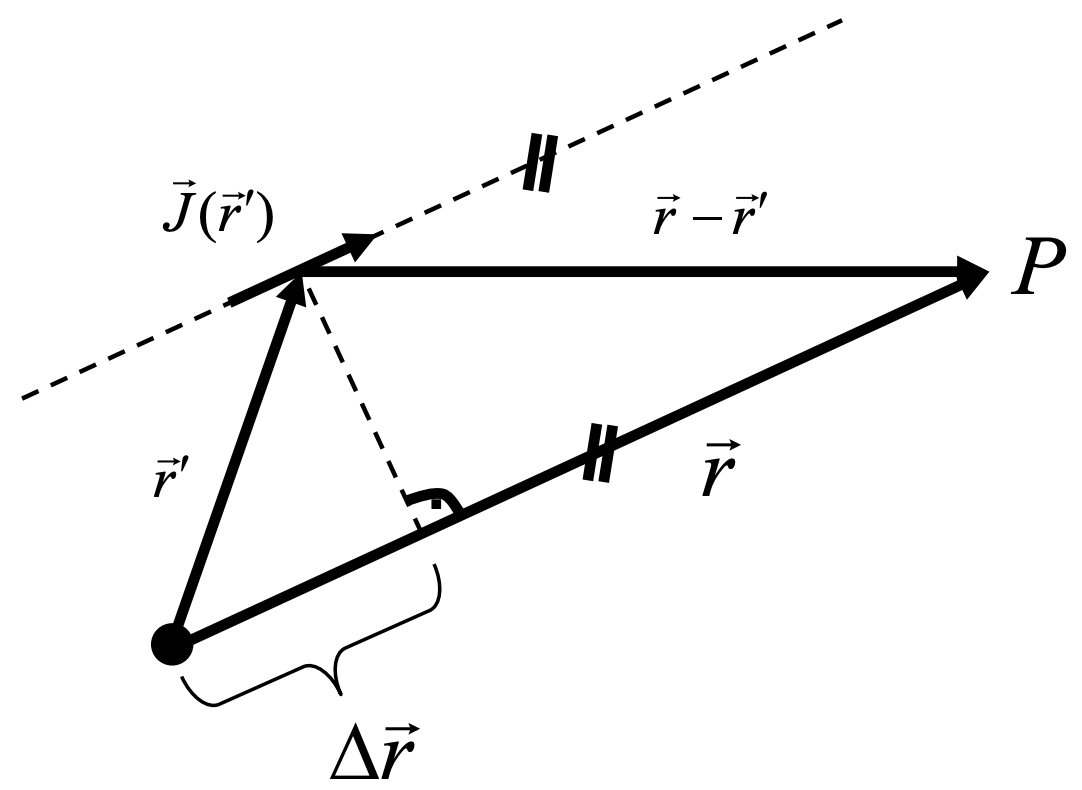
\includegraphics[width = 2.3cm]{./img/fernfeld.png}\end{center}

	Approximiere $\vec{A}(\vec{r})$ unter den Annahmen $r = |\vec{r}|\gg |\vec{r}^{\prime}|$, $r \gg \lambda$.\\
	$\rightarrow$ $|\vec{r} - \vec{r}^{\prime}| \approx r$ im Nenner, und $|\vec{r} - \vec{r}^{\prime}| \approx r - \frac{\vec{r}\cdot\vec{r}^{\prime}}{r}$ im Exp.\\

	\begin{emphbox}
		$\begin{aligned}
			&\vec{A}(\vec{r})=\mu \frac{\mathrm{e}^{-j k r}}{4 \pi r} \iiint\limits_{V} \vec{J}\left(\vec{r}^{\prime}\right) \mathrm{e}^{+j k \frac{\vec{r}\cdot \vec{r}^{\prime}}{r} } d v^{\prime} \\
			&\vec{F}(\vec{r})=\varepsilon \frac{\mathrm{e}^{-j k r}}{4 \pi r} \iiint\limits_{V} \vec{M}\left(\vec{r}^{\prime}\right) \mathrm{e}^{+j k \frac{\vec{r}\cdot \vec{r}^{\prime} }{r}} d v^{\prime}
			\end{aligned}$
	\end{emphbox}

	\begin{emphbox}
		Rotationsoperator im Fernfeld:\\
		$\nabla \times \vec{A} \approx -jk \vec{e}_r \times \vec{A}$\\
		Divergenzoperator im Fernfeld:\\
		$\nabla \cdot \vec{A} \approx -jk \vec{e}_r \cdot \vec{A}$\\
	\end{emphbox}
	\textbf{Sphärische Feldkomponenten im Fernfeld}:
	\begin{tablebox}{@{\hspace{0mm}}l@{\extracolsep\fill}l@{\hspace{0mm}\extracolsep\fill}}
		Elektrische Ströme: & \\
		
			$H_{r 1}=0$ &  $E_{r 1}=0$ \\
			$H_{\vartheta 1}=\frac{j k}{\mu} A_{\varphi}$ & $E_{\vartheta 1}=-j \omega A_{\vartheta}=Z_{F} H_{\varphi 1}$\\
			$H_{\varphi 1}=-\frac{j k}{\mu} A_{\vartheta}$ & $E_{\varphi 1}=-j \omega A_{\varphi}=-Z_{F} H_{\vartheta 1}$\\

		Magnetische Ströme: & \\
			$E_{r 2}=0 $ & $H_{r 2}=0$\\
			$E_{\vartheta 2}=-\frac{j k}{\varepsilon} F_{\varphi}=Z_{F} H_{\varphi 2} $ & $H_{\vartheta 2}=-j \omega F_{\vartheta}$\\
			$E_{\varphi 2}=\frac{j k}{\varepsilon} F_{\vartheta}=-Z_{F} H_{\vartheta 2}$ & $H_{\varphi 2}=-j \omega F_{\varphi}$\\
	\end{tablebox}
	$Z_F = \sqrt{\frac{\mu}{\varepsilon}} = \frac{\omega\mu}{k}$
\end{sectionbox}

\begin{sectionbox}
	\subsection{TEM Wellen}
	$\vec{H} = \frac{1}{Z_F} \vec{e}_z \times \vec{E}$\\
	$\vec{E} = -Z_F \vec{e}_z \times \vec{H}$\\
	$\vec{E} \perp \vec{H} \perp \vec{e}_z$, $\vec{e}_z$ ist Ausbreitungsrichtung.\\
	Nutze Rechte-Hand-Regel für schnelle Berechnung von Kreuzprodukten.
\end{sectionbox}

\begin{sectionbox}
	\subsection{Smithchart Tricks}

	\textbf{Impedanz $\rightarrow$ Bauteilwert}\\
	$L=\frac{(z_L / j)Z_0}{\omega} \quad C=\frac{1}{(-z_C / j)Z_0\omega}$\\
	\textbf{Admittanz $\rightarrow$ Bauteilwert}\\
	$C=\frac{y_C / j}{Z_0 \omega} \quad L = \frac{Z_0}{(-y_L / j) \omega}$\\
\end{sectionbox}
% ======================================================================
% End
% ======================================================================
\end{document}
